%!TeX encoding = UTF-8 Unicode
\documentclass{article}
\usepackage[pdftex]{graphicx} %for embedding images
\usepackage{url} %for proper url entries
\usepackage[bookmarks, colorlinks=false, pdfborder={0 0 0}, pdftitle={Final Report - Recognition Spring 2021}, pdfauthor={Nhut-Nam Le}, pdfsubject={Recognition}, pdfkeywords={report, exercises}]{hyperref} %for creating links in the pdf version and other additional pdf attributes, no effect on the printed document
%\usepackage[final]{pdfpages} %for embedding another pdf, remove if not required
\usepackage[utf8]{inputenc}
\usepackage[vietnamese]{babel}
\usepackage{float}
\usepackage{fancyhdr}
\usepackage{pythonhighlight}
\usepackage[left=3cm, right=3cm, top=2cm, bottom=2cm]{geometry}
\usepackage{parskip}
\usepackage{tikz}
\usepackage{hyperref}
\usepackage[]{algorithm2e}
\usepackage[noend]{algpseudocode}
\usepackage{amsmath}
\usepackage{amsfonts}
\usepackage{hyperref}
\usepackage{listings}
\usepackage{color}


\definecolor{dkgreen}{rgb}{0,0.6,0}
\definecolor{gray}{rgb}{0.5,0.5,0.5}
\definecolor{mauve}{rgb}{0.58,0,0.82}

\newcommand\T{\rule{0pt}{2.6ex}}       % Top strut
\newcommand\B{\rule[-1.2ex]{0pt}{0pt}} % Bottom strut

\newcommand{\foo}{\hspace{-2.3pt}$\bullet$ \hspace{5pt}}

\lstset{frame=tb,
	language=Java,
	aboveskip=3mm,
	belowskip=3mm,
	showstringspaces=false,
	columns=flexible,
	basicstyle={\small\ttfamily},
	numbers=none,
	numberstyle=\tiny\color{gray},
	keywordstyle=\color{blue},
	commentstyle=\color{dkgreen},
	stringstyle=\color{mauve},
	breaklines=true,
	breakatwhitespace=true,
	tabsize=3
}

\usepackage{tikz}
\usepackage{sidecap}
\usetikzlibrary{matrix}
\usetikzlibrary{positioning}
\usetikzlibrary{backgrounds}
\usetikzlibrary{arrows.meta}
\usetikzlibrary{decorations.pathreplacing}

\newcommand\numRowsK{3}
\newcommand\numColsK{3}
\newcommand{\K}[2]{% #1: row, #2: col
	\edef\Kcol##1##2##3{###2}%
	\edef\Krow##1##2##3{\noexpand\Kcol###1}%
	\Krow
	{1 0 1}
	{0 1 0}
	{1 0 1}%
}

\newcommand{\convoutionpicture}[2]{% #1: row to be highlighted, #2: colum to be highlighted
	\begin{tikzpicture}
		% ------- style -------
		\tikzset{%
			parenthesized/.style={%
				left delimiter  = (,
				right delimiter = ),
			},
			node distance = 10mu,
		}
		
		% ------- equation -------
		\matrix[matrix of math nodes, parenthesized, ampersand replacement=\&] (I) {
			0 \& 1 \& 1 \& 1 \& 0 \& 0 \& 0 \\
			0 \& 0 \& 1 \& 1 \& 1 \& 0 \& 0 \\
			0 \& 0 \& 0 \& 1 \& 1 \& 1 \& 0 \\
			0 \& 0 \& 0 \& 1 \& 1 \& 0 \& 0 \\
			0 \& 0 \& 1 \& 1 \& 0 \& 0 \& 0 \\
			0 \& 1 \& 1 \& 0 \& 0 \& 0 \& 0 \\
			1 \& 1 \& 0 \& 0 \& 0 \& 0 \& 0 \\
		};
		
		\node (*) [right = of I] {${}*{}$};
		
		\def\Kmatrix{}
		\foreach \row in {1, ..., 3} {
			\gdef \sep {}
			\foreach \col in {1, ..., 3} {%
				\xdef \Kmatrix {\unexpanded\expandafter{\Kmatrix}\unexpanded\expandafter{\sep}\noexpand \K{\row}{\col}}
				\gdef \sep { \& }
			}
			\xdef \Kmatrix {\unexpanded\expandafter{\Kmatrix}\noexpand\\}
		}
		\matrix[matrix of math nodes, parenthesized, ampersand replacement=\&] (K) [right = of *] {
			\Kmatrix
		};
		
		\node (=) [right = of K] {${}={}$};
		
		\matrix[matrix of math nodes, parenthesized, ampersand replacement=\&] (I*K) [right = of {=}] {
			1 \& 4 \& 3 \& 4 \& 1 \\
			1 \& 2 \& 4 \& 3 \& 3 \\
			1 \& 2 \& 3 \& 4 \& 1 \\
			1 \& 3 \& 3 \& 1 \& 1 \\
			3 \& 3 \& 1 \& 1 \& 0 \\
		};
		
		% ------- highlighting -------
		\def\rowResult{#1}
		\def\colResult{#2}
		
		\begin{scope}[on background layer]
			\newcommand{\padding}{2pt}
			\coordinate (Is-nw) at ([xshift=-\padding, yshift=+\padding] I-\rowResult-\colResult.north west);
			\coordinate (Is-se) at ([xshift=+\padding, yshift=-\padding] I-\the\numexpr\rowResult+\numRowsK-1\relax-\the\numexpr\colResult+\numColsK-1\relax.south east);
			\coordinate (Is-sw) at (Is-nw |- Is-se);
			\coordinate (Is-ne) at (Is-se |- Is-nw);
			
			\filldraw[red,   fill opacity=.1] (Is-nw) rectangle (Is-se);
			\filldraw[green, fill opacity=.1] (I*K-\rowResult-\colResult.north west) rectangle (I*K-\rowResult-\colResult.south east);
			
			\draw[blue, dotted] 
			(Is-nw) -- (K.north west)
			(Is-se) -- (K.south east)
			(Is-sw) -- (K.south west)
			(Is-ne) -- (K.north east)
			;
			\draw[green, dotted] 
			(I*K-\rowResult-\colResult.north west) -- (K.north west)
			(I*K-\rowResult-\colResult.south east) -- (K.south east)
			(I*K-\rowResult-\colResult.south west) -- (K.south west)
			(I*K-\rowResult-\colResult.north east) -- (K.north east)
			;
			
			\draw[blue,  fill=blue!10!white] (K.north west) rectangle (K.south east);
			
			\foreach \row [evaluate=\row as \rowI using int(\row+\rowResult-1)] in {1, ..., \numRowsK} {%
				\foreach \col [evaluate=\col as \colI using int(\col+\colResult-1)] in {1, ..., \numColsK} {%
					\node[text=blue] at (I-\rowI-\colI.south east) [xshift=-.3em] {\tiny$\times \K{\row}{\col}$};
				}
			}
		\end{scope}
		
		% ------- labels -------
		\tikzset{node distance=0em}
		\node[below=of I] (I-label) {$I$};
		\node at (K |- I-label)     {$K$};
		\node at (I*K |- I-label)   {$I*K$};
	\end{tikzpicture}%
}

\setlength{\parindent}{15pt}
\setlength{\headheight}{15.2pt}
\pagestyle{fancy}
\lhead[<even output>]{NHẬN DẠNG}
\rhead[<even output>]{BÁO CÁO ĐỒ ÁN CUỐI KỲ}
\title{research-outline}
\author{Nhut-Nam Le}
\date{2021}
\begin{document}
	
\definecolor{c1}{HTML}{9ACFC6}
\definecolor{c2}{HTML}{DABBD6}
\definecolor{c3}{HTML}{CBDCB9}
\definecolor{c4}{HTML}{9AC3E1}
\definecolor{c5}{HTML}{DEBBA5}
\definecolor{c6}{HTML}{C4DDE5}
\newcommand*{\xMin}{0}%
\newcommand*{\xMax}{6}%
\newcommand*{\yMin}{0}%
\newcommand*{\yMax}{4}%

\newcommand*{\xMinR}{9.5}%
\newcommand*{\xMaxR}{12.5}%
\newcommand*{\yMinR}{1}%
\newcommand*{\yMaxR}{3}%


	\begin{titlepage}
		\begin{center}
			% Top of the page
			\large{\textbf{ĐẠI HỌC KHOA HỌC TỰ NHIÊN, ĐHQG-HCM\\KHOA CÔNG NGHỆ THÔNG TIN\\BỘ MÔN KHOA HỌC MÁY TÍNH}}\\
			
\includegraphics[width=0.75\textwidth]{images/khtn.png}\\
			% Title
			%\large \textbf{BÁO CÁO ĐỒ ÁN CUỐI KỲ}\\[0.1in]
			\huge \textbf{NHẬN DẠNG}\\[0.1in]
			\huge \textbf{BÁO CÁO ĐỒ ÁN CUỐI KỲ}\\[0.1in]
			\vfill
			\normalsize
			% Submitted by
			\normalsize
			% Lecturers
			\textbf{Giảng viên lý thuyết}\\
			{\textbf{PGS. TS.} Lê Hoàng Thái}\\[0.1in]
			% Teacher Assistant
			\textbf{Giảng viên hướng dẫn}\\
			\vspace{0.1in}
			{Lê Thanh Phong, Nguyễn Ngọc Thảo}\\[0.1in]
			\textbf{Sinh viên thực hiện} \\
			\vspace{0.1in}
			{Nguyễn Hoàng Đức, Lê Nhựt Nam, Nguyễn Viết Dũng}\\[0.1in]
			% Date time when written report
			\vfill
			Tháng 7 năm 2021
		\end{center}
	\end{titlepage}
	\newpage
	% End Title4
	
	\pagenumbering{roman} %numbering before main content starts
	\cleardoublepage
	%\pagebreak
	\phantomsection
	\addcontentsline{toc}{section}{Lời cảm ơn}
	\section*{Lời cảm ơn}
	\vspace{1.0in}
	\begingroup
	\setlength{\parindent}{0pt}
	\qquad Trong quá trình thực hiện đồ án này, chúng em đã nhận được rất nhiều sự giúp đỡ cũng như hỗ trợ từ các thầy cô Trường Đại học Khoa học Tự nhiên, ĐHQG-HCM và các bạn bè trong lớp Nhận dạng. Chúng em xin bày tỏ lòng cảm ơn chân thành đến mọi người vì đã giúp đỡ hướng dẫn, chỉ bảo rất tận tình.
	
	Đặc biệt, chúng em xin bày tỏ lòng biết ơn sâu sắc đến các thầy cô khoa Công nghệ Thông tin, cụ thể hơn là thầy Hoàng Thái, thầy Thanh Phong và cô Ngọc Thảo, dẫn đã giảng dạy rất nhiệt, cung cấp nhiều slides, tài nguyên học tập cần thiết, tạo điều kiện tốt nhất để chúng em có thể hoàn thành được đồ án này.
	
	Trong lúc viết báo cáo này, chúng em không thể tránh khỏi nhiều thiếu sót, hy vọng mong nhận được góp ý từ thầy để chúng em tiếp tục hoàn thiện hơn đối với đồ án này, cũng như rút kinh nghiệm cho những đồ án, những báo cáo kế tiếp.
	
	\vspace{1.0in}
	\textbf{Đại học Khoa học Tự nhiên, ĐHQG-HCM.}\\
	Nguyễn Hoàng Đức, Lê Nhựt Nam, Nguyễn Viết Dũng\\
	Tháng 5 năm 2021\\
	\endgroup
	\newpage
	\tableofcontents
	\newpage
	\pagenumbering{arabic} %reset numbering to normal for the main content
	\setcounter{secnumdepth}{0}
	
	\section{A. Câu hỏi lý thuyết}
	
	\subsection{A.1 Kiến thức về Local Binary Patterns (LBP)}
	
	\subsubsection{a. Trình bày đặc trưng mẫu nhị phân cục bộ $\text{LBP}_{\text{P,R}}$}
	\textbf{(1) Phương pháp xác định giá trị}\newline
	
	\qquad Phương pháp xác định giá trị LBP sơ khai: Được tính toán bằng cách tại mỗi điểm ảnh, xét 8 điểm xung quanh nó
	\begin{itemize}
		\item Bước 01: Các điểm xung quanh có giá trị nhỏ hơn điểm đang xét sẽ được đánh dấu là 0, lớn hơn điểm đang xét sẽ được đánh dấu là 1.
		\item Bước 02: Sau đó, các giá trị sau khi tính toán phân ngưỡng ở trên sẽ được nhân với ma trận trọng số và được sử dụng để tính giá trị LBP của điểm đang xét.
	\end{itemize}

	$$\begin{bmatrix}1 & 2 & 4 \\128 & & 8\\64 & 32 & 16\end{bmatrix}$$
	
	\begin{figure}[H]
		\centering
		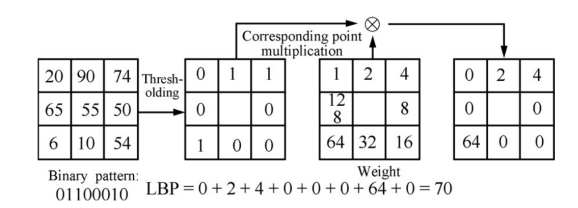
\includegraphics[width=0.75\linewidth]{images/orginal_lbp.png}
		\caption{Mô tả quá trình thực hiện LPB}
		\label{fig:writing-thesis}
	\end{figure}
	Phương pháp xác định giá trị LBP cải tiến: Xét các điểm thuộc đường tròn với tâm là điểm đang xét. Ta gọi $(P,R)$ là vùng lân cận gồm $P$ điểm trên một đường tròn bán kinh $R$
	
	\begin{equation}
		T = t(g_c, g_0, ..., g_{p-1})
	\end{equation}

	Trong đó:
	\begin{itemize}
		\item $g_c$ và $(g_0, ..., g_{p-1})$ là giá trị trên ảnh xám của điểm trung tâm và các điểm trên đường tròn bán kính $R$
	\end{itemize}

	Ta có thể xấp xỉ công thức trên bằng cách lấy từng điểm trên đường tròn bán kinh $R$ trừ đi giá trị trung tâm $g_c$ do các giá trị chỉ thể hiện cường độ sáng của điểm ảnh.
	
	\begin{equation}
		T \approx t(g_0 - g_c, g_1 - g_c, ..., g_{p-1} - g_c)
	\end{equation}

	Để không bị ảnh hưởng bởi các giá trị của các điểm ảnh, chuẩn hoá công thức trên bằng việc xét dấu
	
	\begin{equation}
		T \approx t(sign(g_0 - g_c), sign(g_1 - g_c), ..., sign(g_{p-1} - g_c))
	\end{equation}
		
	Trong đó:
	$$sign(x) = \begin{cases}1, x \geq 0\\ 0, x < 0\end{cases}$$
	
	Giá trị LBP được tính như sau:
	
	\begin{equation}
		LBP_{P, R} = \sum_{i=0}^{p-1} sign(g_i-g_c) \times 2^i
	\end{equation}

	\textbf{(2) Ưu điểm}\newline
	\begin{itemize}
		\item Bất biến đối với bất kỳ phép biến đổi đơn điệu nào trên ảnh xám (grayscale) nên hiệu quả cho việc làm giảm tỷ lệ từ chối sai (FRR) cho mỗi đối tượng, khi đối tuợng đó được chụp tại những điều kiện sáng/ tối khác nhau
		\item Lượng tử hoá vector là không cần thiết
		\item Tính toán một cách đơn giản
	\end{itemize}

	\begin{figure}[H]
		\centering
		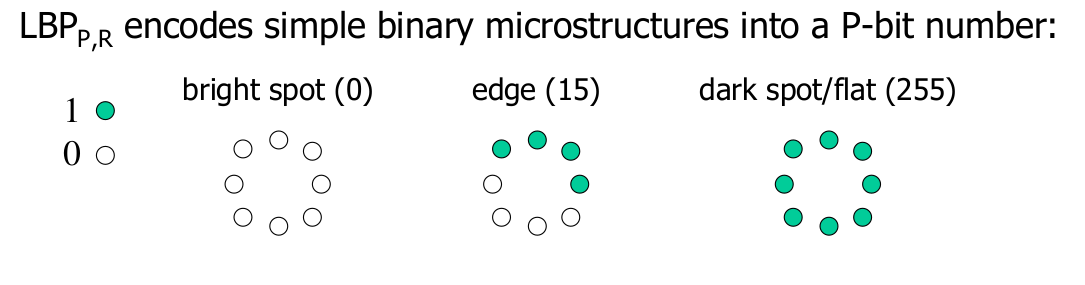
\includegraphics[width=0.75\linewidth]{images/lbp_pr.png}
		\caption{Mô tả quá trình thực hiện LPB}
		\label{fig:writing-thesis}
	\end{figure}

	\textbf{(3) Nhược điểm}\newline
	
	Chưa quan tâm đến phép quay, đặc trưng LBP áp dụng trên hình ảnh xoay của cùng một đối tượng sẽ tạo ra các giá trị khác nhau.
	
	\begin{figure}[H]
		\centering
		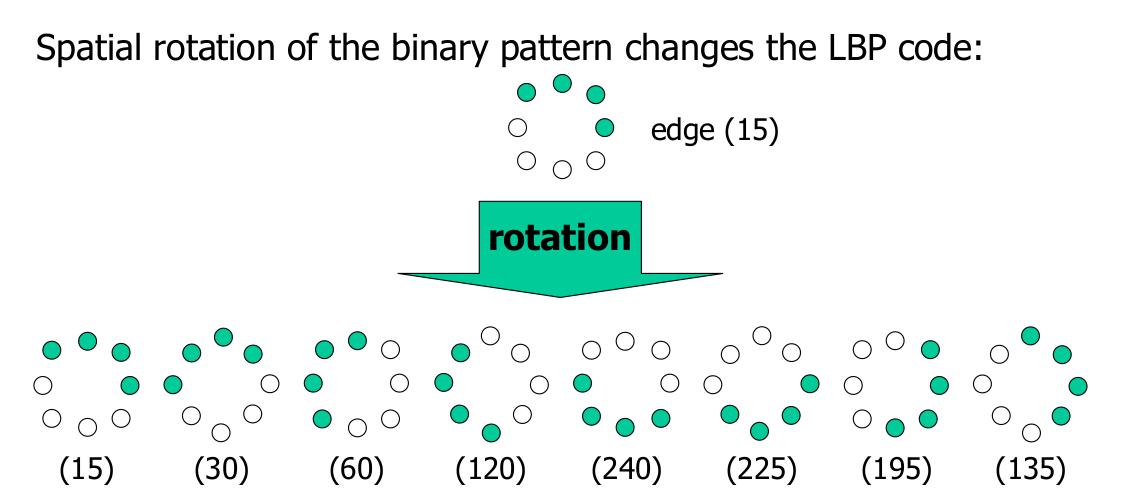
\includegraphics[width=0.75\linewidth]{images/stuck_lbp_pr.png}
		\caption{Ảnh hưởng của phép xoay lên đặc trưng LBP}
		\label{fig:writing-thesis}
	\end{figure}
	
	Có vấn đề khi số điểm lân cận tăng quá cao, giá trị LBP sẽ tăng lên rất cao
	
	\subsubsection{b. Sự khác biệt giữá đặc trưng $\text{LBP}_{\text{P,R}}$ so với đặc trưng $\text{LBP}_{\text{P,R}^{\text{ri}}}$}
	
	\qquad Đặc trưng $LBP_{(P, R)^{ri}}$ khắc phục nhược điểm của đặc trưng $LBP_{(P, R)}$: bất biến với phép xoay, chọ giá trị nhỏ nhất để đại diện cho tất cả các ảnh xoay (mỗi ảnh được xoay theo hướng của vòng tròn luợng giác một góc xác định cho trước)
	
	
	Mã nhị phân phát sinh bởi LBP được xoay trong vòng tròn, theo hướng bên phải, một cách liên tục để đạt được giá trị nhỏ hơn cho mã nhị phân.
	
	Ví dụ: 11101000 được dịch bit thành 01110100, sau đó thành 00111010, và cuối cùng là  00011101 sẽ là giá trị nhỏ nhất
	
	\begin{figure}[H]
		\centering
		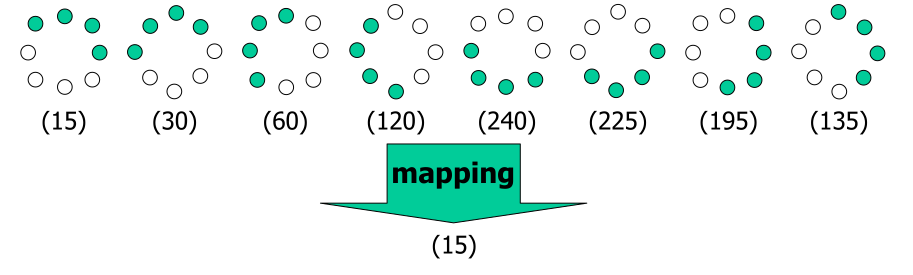
\includegraphics[width=0.75\linewidth]{images/lbp_ri.png}
		\caption{Đặc trưng LBP PR ri}
		\label{fig:writing-thesis}
	\end{figure}
	
	Để đạt được bất biến với phép quay, một hàm bất biến xoay của LBP được định nghĩa bằng 
	
	\begin{equation}
		LBP_{(P, R)^{ri}} = min(ROR(LBP_{(P, R)^{ri}}, i)i = 0, 1, ..., P-1)
	\end{equation}
	
	Trong đó, ROR là hàm xoay có tác dụng thay đổi chuỗi nhị phân thu được từ các điểm mẫu lần lượt. Sau khi tính toán hết giá trị LBP cho mỗi chuỗi, giá trị nhỏ nhất sẽ được chọn để biểu diễn mẫu kết cấu đó. Vì thế, thay vì phải xử lý 256 mẫu khác nhau cho $LBP_{8, 1}$, ta chỉ cần 36 mẫu khác nhau
	
	\begin{figure}[H]
		\centering
		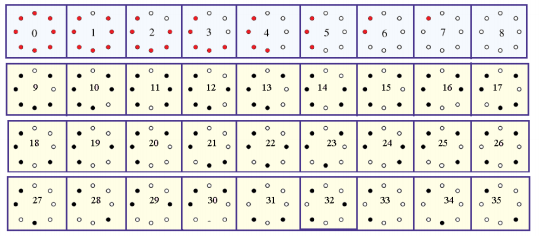
\includegraphics[width=0.75\linewidth]{images/lbp_rotation_invariant.png}
		\caption{LBP Rotation Invariance}
		\label{fig:writing-thesis}
	\end{figure}
	
	
	\subsubsection{c. Sự khác biệt giữá đặc trưng $\text{LBP}_{\text{P,R}^{\text{riu2}}}$ so với đặc trưng $\text{LBP}_{\text{P,R}^{\text{ri}}}$}
	Đặc trưng $\text{LBP}_{\text{P,R}^{\text{riu2}}}$ cải tiến so với đặc trưng $\text{LBP}_{\text{P,R}^{\text{ri}}}$ bằng cách sử dụng khái niệm "mẫu đồng phục" - "Uniform Patterns"
	
	\begin{figure}[H]
		\centering
		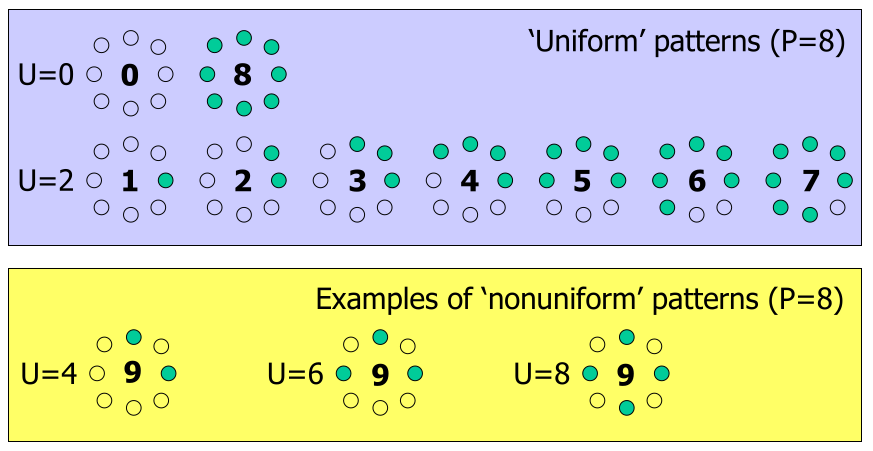
\includegraphics[width=0.75\linewidth]{images/lbp_uniform_2.png}
		\caption{Uniform Patterns}
		\label{fig:writing-thesis}
	\end{figure}

	\begin{figure}[H]
		\centering
		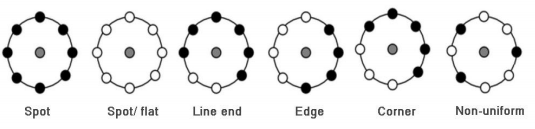
\includegraphics[width=0.75\linewidth]{images/lbp_uniform_types.png}
		\caption{Hình ảnh nguyên thủy được nắm bắt bởi mẫu LBP}
		\label{fig:writing-thesis}
	\end{figure}
	
	Để kiểm tra một mẫu kết cấu có phải là "Uniform Patterns" hay không, ta áp dụng công thức
	
	\begin{equation}
		U(LBP_{P,R}) = |sign(g_{p-1} - g_c) - sign(g_0 - g_c)| + \sum_{i=1}^{p-1}|sign(g_i - g_c) - sign(g_{i-1} - g_c)|
	\end{equation}
	Khi $U \leq 2$, mẫu kết cấu gọi là "Uniform Patterns", ngược lại là "Non-Uniform Patterns"
	
	Công thức tính "Uniform Patterns"
	\begin{equation}
		LBP_{P, R}^{riu2} = \begin{cases}\sum_{i=0}^{p-1}(g_i - g_c), \text{ if } U(LBP_{P, R}) \leq 2\\P+1, \text{otherwise}\end{cases}
	\end{equation}

	\begin{figure}[H]
		\centering
		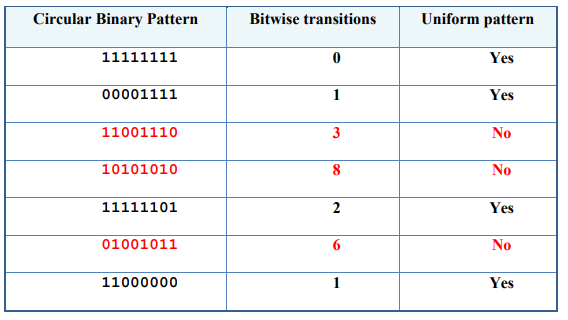
\includegraphics[width=0.75\linewidth]{images/example_uniform_non_uniform.png}
		\caption{Ví dụ Uniform và Non-Uniform LBP Patterns}
		\label{fig:writing-thesis}
	\end{figure}

	\subsubsection{d. Trình bày một biến thể của LBP}
	\qquad Trong phần này, chúng em xin được trình bày một biến thể khá kinh điển của LBP, ILBP hay Improved Local Binary Pattern được trình bày trong bài báo Face Detection Using Improved LBP Under Bayesian Framework bởi Hongliang Jin, Qingshan Liu, Hanqing Lu, Xiaofeng Tong đến từ National Lab of Pattern Recognition, Institute of Automation, Chinese Academy of Sciences, China được công bố tại hội nghị Third International Conference on Image and Graphics (ICIG'04) năm 2004
	
	Đặc trưng ILBP là một cải tiến của đặc trưng LBP, xem xét cả dáng cục bộ (local shape) và thông tin kết cấu (texture information) thay vì thông tin xám thô (raw grayscale information) và nó cực kỳ tốt với sự thay đổi ánh sáng (illumination variation).\newline
	\textbf{(1) Phương pháp xác định giá trị}\newline
	Với một tập $P$ lân cận và một đường tròn bán kính $R$, ta dễ dàng tính được hiệu số giữa pixel trung tâm (central pixel) $g_c$ và lân cận của nó $\{g_0, ..., g_{p-1}\}$
	\begin{gather*}
		LBP_{P,R} = \sum_{i=0}^{P-1}s(g_i - g_c)^2\\
		s(x) = \begin{cases}
			1, x > 0\\
			0, x \leq 0
		\end{cases}
	\end{gather*}
	\begin{figure}[H]
		\centering
		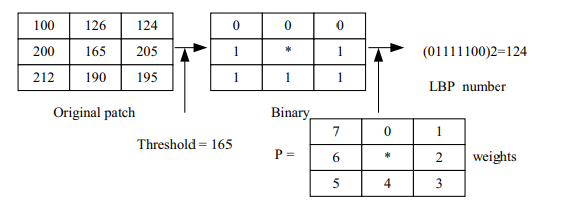
\includegraphics[width=0.75\linewidth]{images/cau_d.png}
		\caption{Mô tả quá trình thực hiện LPB}
		\label{fig:writing-thesis}
	\end{figure}
	Đặc trưng Improved Local Binary Pattern từ ý tưởng ánh xạ giá trị điểm ảnh sang một khoảng giá trị mới, có thể được khai triển như sau:
	\begin{gather*}
		LBP_{P,R} = \sum_{i=0}^{P-1}s(g_i-m)2^i+s(g_c - m)2^P\\
		s(x) = \begin{cases}
			1, x > 0\\
			0, x \leq 0
		\end{cases}\\
		m = \frac{1}{P+1}\left(\sum_{i=0}^{P-1}g_i + g_c\right)
	\end{gather*}
	\begin{figure}[H]
		\centering
		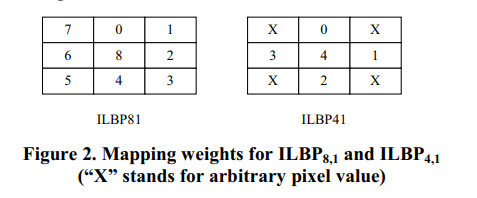
\includegraphics[width=0.75\linewidth]{images/cau_d_1.png}
		\caption{Ánh xạ trọng số cho ILBP 8,1 và ILBP 4,1}
		\label{fig:writing-thesis}
	\end{figure}
	
	\begin{figure}[H]
		\centering
		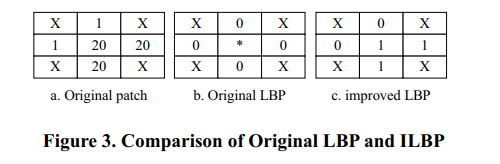
\includegraphics[width=0.75\linewidth]{images/cau_d_2.png}
		\caption{So sánh giữa đặc trưng LBP và ILBP}
		\label{fig:writing-thesis}
	\end{figure}

	\textbf{(2) Ưu điểm và nhược điểm, trên cơ sở so sánh LBP}\newline
	Về ưu điểm của ILBP:
	\begin{itemize}
		\item Giữa được cấu trúc cục bộ trong một số hoàn cảnh nhất định. Khi sử dụng LBP truyền thống, ta chỉ có thể sử dụng $2^8 = 256$ trong tổng số 511 patterns từ một patch $3 \times 3$
		\item ILBP xem xét nhiều hơn pixel trung tâm, trong đa số trường hợp, pixel trung tâm có nhiều thông tin hơn những lân cận của nó. Vì thế, trong ILBP, pixel trung tâm được mang trọng số lớn nhất
	\end{itemize}
	Về nhược điểm ILBP
	\begin{itemize}
		\item Những hình ảnh có chứa nguồn sáng cực mạnh khi sử dụng phương pháp này sẽ có kết quả không cao vì những thông tin cấu trúc đã bị mất mát
	\end{itemize}
		
	
	\subsection{A.2 Kiến thức về Principal Component Analysis (PCA) và Linear Discriminant Analysis (LDA)}
	
	\subsubsection{a. Các bước thực hiện của giải thuật phân tích thành phần chính PCA}
	\qquad Tư tưởng chính của PCA là đem chiếu dữ liệu sang một miền mới có số chiều d nhỏ hơn số chiều ở miền gốc là D, sao cho phương sai của dữ liệu sau khi được chiếu là lớn nhất có thể.\newline
	Thuật toán PCA:\newline
	Input: $D = {x_1, x_2, ..., x_n}, x_i \in R^{D}$\newline
	Output: W \newline
	\textbf{Bước 1}. Xây dựng vector trung bình $\mu$ 
	$$\mu = \frac{1}{n}\sum_{i=1}^{n}x_i$$
	\textbf{Bước 2}. Xây dựng ma trận hiệp phương sai $S$ 
	$$S = \frac{1}{n}\sum_{i=1}^{n}(x_i - \mu_i)(x_i - \mu_i)^T$$
	\textbf{Bước 3}. Phân rã ma trận hiệp phương sai thành những cặp vector riêng và giá trị riêng
	$$\{w_1, w_2, ..., w_D\}$$ 
	và 	
	$$\lambda_1, \lambda_2, ..., \lambda_D$$
	\textbf{Bước 4}. Sắp xếp các giá trị riêng theo thứ tự giảm dần tương ứng với các vectors riêng 
	$$\{w_1, w_2, ..., w_D\}$$ 
	và 
	$$\lambda_1 \geq \lambda_2 \geq ... \geq \lambda_D$$
	\textbf{Bước 5}. Chọn $k$ vector riêng mà tương ứng với $k$ giá trị riêng lớn nhất, với $k$ là số chiều đặc trưng mới  ($k \leq D$). Ở đây mình sẽ có một cách chọn k sao cho hợp lý với cách dựa vào threshold
	$$\{w_1, w_2, ..., w_k\}$$ 
	và 
	$$\lambda_1 \geq \lambda_2 \geq ... \geq \lambda_k$$
	\textbf{Bước 6}. Xây dưng ma trận hình chiếu $W$ từ $k$ vector riêng 
	$$W = [w_1, w_2, ..., w_k]^T$$
	\textbf{Bước 7}: Ta có một phép biến đổi tuyến tính (linear transformation) $R^N \rightarrow R^k$ thực hiện giảm chiều (dimensionality reduction)
	$$
	\begin{bmatrix}
		b_1 \\
		b_2 \\
		... \\
		b_k \\
	\end{bmatrix} = 
	\begin{bmatrix}
		w_1^T \\
		w_2^T \\
		... \\
		w_k^T \\
	\end{bmatrix}(x- \bar{x}) = W^T(x- \bar{x})
	$$
	Để chọn được giá trị $k$, chúng ta có thể sử dụng tiêu chí sau:
	$$\frac{\sum_{i=1}^k\lambda_i}{\sum_{i=1}^N\lambda_i} > \text{threshold}$$
	Trong đó: threshold là một người mà chúng ta muốn, có thể là 0.9, 0.95\newline
	Ví dụ: Cho dữ liệu \newline
	$$
	X = \begin{bmatrix}
		7 & 4& 6& 8& 8 &7& 5& 9 &7& 8 \\
		4 &1 &3& 6& 5& 2& 3& 5& 4 &2\\
		3 &8 &5 &1&7& 9& 3& 8& 5& 2
	\end{bmatrix}
	$$
	\textbf{Bước 01}: Tính toán vector trung bình
	$$\text{mean\_vector} = [6.9, 3.5, 5.1]$$
	\textbf{Bước 02}: Xây dựng ma trận hiệp phương sai
	$$
	C = \begin{bmatrix}
		2.32 & 1.61 & -0.43\\
		1.61 & 2.5 & -1.278\\
		-0.43 & -1.278 & 7.878\\
	\end{bmatrix}
	$$
	\textbf{Bước 03}: Phân rã ma trận hiệp phương sai thành những cặp vector riêng và giá trị riêng
	$$w_1 = [-0.7012, 0.7075, 0.0841], \lambda_1 = 0.7499$$
	$$w_2 = [0.699, 0.6609, 0.2731], \lambda_2 = 3.6761$$
	$$w_3 = [-0.1376, -0.2505, 0.9583], \lambda_3 = 8.2739$$
	\textbf{Bước 04}: Sắp xếp các giá trị riêng theo thứ tự giảm dần tương ứng với các vectors riêng 
	$$w_3 = [-0.1376, -0.2505, 0.9583], \lambda_3 = 8.2739$$
	$$w_2 = [0.699, 0.6609, 0.2731], \lambda_2 = 3.6761$$
	$$w_1 = [-0.7012, 0.7075, 0.0841], \lambda_1 = 0.7499$$
	\textbf{Bước 05}: Chọn $k=2$ vector riêng mà tương ứng với $k$ giá trị riêng lớn nhất, với $k$ là số chiều đặc trưng mới  ($k \leq D$). Ở đây mình sẽ có một cách chọn k sao cho hợp lý với cách dựa vào threshold
	$$w_3 = [-0.1376, -0.2505, 0.9583], \lambda_3 = 8.2739$$
	$$w_2 = [0.699, 0.6609, 0.2731], \lambda_2 = 3.6761$$
	\textbf{Bước 06}: Xây dưng ma trận hình chiếu $W$ từ $k=2$ vector riêng 
	$$W = 
	\begin{bmatrix}
		-0.1376 & 0.699\\
		-0.2505 & 0.6609\\
		0.9583 & 0.2731\\
	\end{bmatrix}
	$$
	\textbf{Bước 7}: Giảm chiều dữ liệu
	$$
	\begin{bmatrix}
		b_1 \\
		b_2 \\
		... \\
		b_k \\
	\end{bmatrix} = 
	\begin{bmatrix}
		w_1^T \\
		w_2^T \\
		... \\
		w_k^T \\
	\end{bmatrix}(x- \bar{x}) = W^T(X- \bar{X})
	$$
	
	$$
	\begin{bmatrix}
		-0.1376 & -0.2505 & 0.9583\\
		0.699 & 0.6609 & 0.2731
	\end{bmatrix} 
	\begin{bmatrix}
		0.1 & -2.9 & -0.9 & 1.1 & 1.1 & 0.1 & -1.9 & 2.1 & 0.1 & 1.1\\
		0.5 & -2.5 & -0.5 & 2.5 & 1.5 & -1.5 & -0.5 & 1.5 & 0.5 & -1.5\\
		-2.1 & 2.9 & -0.1 & -4.1 & -1.9 & -3.9 & -2.1 & 2.9 & -0.1 & -3.1\\
	\end{bmatrix} 
	$$
	$$
	=
	\begin{bmatrix}
		-2.15 & 3.80 & 0.15 & -4.7 & 1.29 & 4.09 & -1.63 & 2.11 & -0.23 & -2.75\\
		-0.17 & -2.89 & -0.999 & 1.30 & 2.28 & 0.14 & -2.23 & 3.25 & 0.37 & -1.07\\
	\end{bmatrix}
	$$
	Tính $\hat{X}$
	$$\hat{X} = W^T.Y + \bar{X}
	=\begin{bmatrix}
		7.075 & 4.3582 & 6.1891 & 8.4573 & 8.3152 & 6.4364 & 5.5633 & 8.8818 & 7.1931 & 6.5306\\
		3.9244 & 0.6388 & 2.8094 & 5.5389 & 4.6822 & 2.5682 & 2.4320 & 5.1129 & 3.8054 & 3.4814 \\
		2.9910 & 7.9570 & 4.9773& 0.9451& 6.9622& 9.6076& 2.9324& 8.0142 &4.9768 &7.1762\\
	\end{bmatrix}
	$$
	$$MSE = \frac{1}{10}\sum_{i=1}^{10}(X_i - \hat{X}_i)^2 = 0.67493$$
	\subsubsection{b. Các bước chính của giải thuật tách lớp tuyến tính LDA}
	\qquad Tư tưởng chính của giải thuật tách lớp tuyến tính LDA là cực tiểu khoảng cách các phần tử trong cùng một lớp (distance within-class) và cực đại khoảng cách các phần tử nằm khác lớp với nhau (distance between-class). Giải thuật là có giám sát bởi vì dữ liệu đầu vào có dán nhãn trước. Sau đây là phần trình bày các bước chính của giải thuật.\newline
	\textbf{Input - Đầu vào bài toán}: Data labeled $$\mathcal{D} = \{(x_1, y_1), (x_2, y_2), ..., (x_n, y_n)\}, x_i \in \mathcal{R}^D, y_i \in \{c_1, ..., c_k\}$$
	\textbf{Output - Đầu ra}: ma trận chiếu $W$\newline
	Giả sử có $k$ lớp. Đặt $\mu_i$ là vector trung bình của mỗi lớp $i$, với $i = 1, 2, ..., k$\newline
	Đặt $N_i$ là số lượng mẫu trong mỗi lớp thứ  $i$, với $i = 1, 2, ..., k$\newline
	Đặt $N = \sum_{i=1}^kN_i$ là tổng số lượng mẫu\newline
	\textbf{Bước 01}: Với mỗi lớp, tính toán vector trung bình $D$\newline
	\textbf{Bước 02}: Xây dựng ma trận phân tán between-class $S_B$ và ma trận phân tán within-class $S_W$\newline
	Within-class scatter matrix
	$$S_W = \sum_{i=1}^k\sum_{j=1}^{N_i}(x_j - \mu_i)(x_j - \mu_j)^T$$
	Between-class scatter matrix
	$$S_B = \sum_{i=1}^k(\mu_i - \mu)(\mu_i - \mu)^T$$
	$$\mu = \frac{1}{k}\sum_{i=1}^k\mu_i$$
	\textbf{Bước 03}: Tính toán vector riêng và giá trị tương ứng của ma trận $S_W^{-1}S_B$
	$$S_bw_k = \lambda_kS_Ww_k$$
	\textbf{Bước 04}: Sắp xếp những giá trị riêng tương ứng với những vector riêng theo chiều giảm dần\newline
	\textbf{Bước 05}: Chọn $n$ vector riêng tương ứng với $n$ giá trị riêng lớn nhất để xây dựng ma trận biến đổi $D \times D$ chiều $W$, những vector riêng là những cột của ma trận này
	$$
	\begin{bmatrix}
		b_1 \\
		b_2 \\
		... \\
		b_k \\
	\end{bmatrix} = 
	\begin{bmatrix}
		w_1^T \\
		w_2^T \\
		... \\
		w_k^T \\
	\end{bmatrix}(x- \bar{x}) = W^T(x- \bar{x})
	$$
	Bởi vì $S_B$ có hạng lớn nhất là $k-1$, số vector riêng lớn nhất khác 0 là $k-1$\newline
	Trường hợp $S_W^{-1}$ không tồn tại
	- Nếu $S_W$ không là ma trận đơn (non-singular matrix)
	$$S_W^{-1}S_Bw_k = \lambda_kw_k$$
	Trường hợp $S_W^{-1}$ luôn luôn không tồn tại\newline
	- Dùng PCA trước
	$$
	\begin{bmatrix}
		x_1 \\
		x_2 \\
		... \\
		x_N \\
	\end{bmatrix} \longrightarrow PCA \longrightarrow \begin{bmatrix}
		y_1 \\
		y_2 \\
		... \\
		y_K \\
	\end{bmatrix}
	$$
	- Sau đó áp dụng LDA
	$$
	\begin{bmatrix}
		x_1 \\
		x_2 \\
		... \\
		x_N \\
	\end{bmatrix} \longrightarrow LDA \longrightarrow \begin{bmatrix}
		y_1 \\
		y_2 \\
		... \\
		y_{k-1} \\
	\end{bmatrix}
	$$
	Ví dụ bài toán phân lớp với LDA (Bài toán phân lớp với 2 lớp)\newline
	Cho hai lớp \newline
	\begin{itemize}
		\item lớp 1 $\pi_1$: $X_1 = (x_1, x_2) = \{(4,2),(2,4),(2,3),(3,6),(4,4)\}$
		\item lớp 2 $\pi_2$: $X_2 = (x_1, x_2) = \{(9,10),(6,8),(9,5),(8,7),(10,8)\}$
	\end{itemize}	
	Ta có $k = 2$ lớp\newline
	Dặt $\mu_i$ là vector trung bình của mỗi lớp $i$, với $i = 1, ..., k$\newline
	Đặt $N_i$ là số lượng mẫu trong mỗi lớp thứ  $i$, với $i = 1, ..., k$\newline
	Đặt $N = \sum_{i=1}^kN_i$ là tổng số lượng mẫu\newline
	\textbf{Bước 01}: Với mỗi lớp, tính toán vector trung bình $D$ chiều\newline
	Gọi $\mu_1$ và $\mu_2$ là vector trung bình lớp thứ nhất và lớp thứ hai. Ta có:
	\begin{gather*}
		\mu_1 = \frac{1}{N_1}\sum_{x \in \pi_1}x = \frac{1}{5}\left[
		\begin{pmatrix}4\\2\end{pmatrix}
		+ \begin{pmatrix}2\\4\end{pmatrix}
		+ \begin{pmatrix}2\\3\end{pmatrix}
		+ \begin{pmatrix}3\\6\end{pmatrix}
		+ \begin{pmatrix}4\\4\end{pmatrix}
		\right]
		= \begin{pmatrix}3\\3.8\end{pmatrix}
	\end{gather*}
	\begin{gather*}
		\mu_2 = \frac{1}{N_2}\sum_{x \in \pi_2}x = \frac{1}{5}\left[
		\begin{pmatrix}9\\10\end{pmatrix}
		+ \begin{pmatrix}6\\8\end{pmatrix}
		+ \begin{pmatrix}9\\5\end{pmatrix}
		+ \begin{pmatrix}8\\7\end{pmatrix}
		+ \begin{pmatrix}10\\8\end{pmatrix}
		\right]
		= \begin{pmatrix}8.4\\7.6\end{pmatrix}
	\end{gather*}
	\textbf{Bước 02}: Xây dựng ma trận phân tán between-class $S_B$ và ma trận phân tán within-class $S_W$\newline
	Tính ma trận hiệp phương sai của lớp thứ nhất
	\begin{gather*}
		S_1 = \sum_{x \in \pi_1}(x - \mu_1)(x - \mu_1)^T\\
		= \left[\begin{pmatrix}4\\2\end{pmatrix} - \begin{pmatrix}3\\3.8\end{pmatrix}\right]^2
		+ \left[\begin{pmatrix}2\\4\end{pmatrix} - \begin{pmatrix}3\\3.8\end{pmatrix}\right]^2
		+ \left[\begin{pmatrix}2\\3\end{pmatrix} - \begin{pmatrix}3\\3.8\end{pmatrix}\right]^2
		+ \left[\begin{pmatrix}3\\6\end{pmatrix} - \begin{pmatrix}3\\3.8\end{pmatrix}\right]^2
		+ \left[\begin{pmatrix}4\\4\end{pmatrix} - \begin{pmatrix}3\\3.8\end{pmatrix}\right]^2
		\\
		= \begin{pmatrix}1 & -0.25\\-0.25 & 2\end{pmatrix}
	\end{gather*}
	Tính ma trận hiệp phương sai của lớp thứ hai
	\begin{gather*}
		S_2 = \sum_{x \in \pi_2}(x - \mu_2)(x - \mu_2)^T\\
		= \left[\begin{pmatrix}9\\10\end{pmatrix} - \begin{pmatrix}8.4\\7.6\end{pmatrix}\right]^2
		+ \left[\begin{pmatrix}6\\8\end{pmatrix} - \begin{pmatrix}8.4\\7.6\end{pmatrix}\right]^2
		+ \left[\begin{pmatrix}9\\5\end{pmatrix} - \begin{pmatrix}8.4\\7.6\end{pmatrix}\right]^2
		+ \left[\begin{pmatrix}8\\7\end{pmatrix} - \begin{pmatrix}8.4\\7.6\end{pmatrix}\right]^2
		+ \left[\begin{pmatrix}10\\8\end{pmatrix} - \begin{pmatrix}8.4\\7.6\end{pmatrix}\right]^2
		\\
		= \begin{pmatrix}2.3 & -0.3\\-0.3 & 3.3\end{pmatrix}
	\end{gather*}
	Ma trận phân tán between-class $S_B$
	\begin{gather*}
		S_B = (\mu_1 - \mu_2)(\mu_1 - \mu_2)^T = \left[\begin{pmatrix}3\\3.8\end{pmatrix} - \begin{pmatrix}8.4\\7.6\end{pmatrix}\right]\left[\begin{pmatrix}3\\3.8\end{pmatrix} - \begin{pmatrix}8.4\\7.6\end{pmatrix}\right]^T
		= \begin{pmatrix}-5.4\\-3.8\end{pmatrix} \begin{pmatrix}-5.4 &-3.8\end{pmatrix}
		=  \begin{pmatrix}29.16 & 20.52\\20.52 & 14.44\end{pmatrix}
	\end{gather*}
	Ma trận phân tán within-class $S_W$
	\begin{gather*}
		S_W = S_1 S_2 = \begin{pmatrix}1 & -0.25\\-0.25 & 2\end{pmatrix} + \begin{pmatrix}2.3 & -0.05\\-0.05 & 3.3\end{pmatrix} = \begin{pmatrix}3.3 & -0.3\\-0.3 & 5.5\end{pmatrix}
	\end{gather*}
	\textbf{Bước 03}: Tính toán vector riêng và giá trị tương ứng của ma trận $S_W^{-1}S_B$
	$$S_W^{-1}S_Bw_k = \lambda_kw_k$$
	Ta có:
	\begin{gather*}
		det(S_W^{-1}S_B - \lambda I_n) = 0\\
		\Rightarrow det\left(\begin{pmatrix}2.3 & -0.3\\-0.3 & 3.3\end{pmatrix}^{-1} \begin{pmatrix}29.16 & 20.52\\20.52 & 14.44\end{pmatrix} - \lambda\begin{pmatrix}1 & 0\\0 & 1\end{pmatrix}\right) = 0\\
		\Rightarrow det\left(\begin{pmatrix}0.305 & 0.017\\0.017 & 0.183\end{pmatrix}\begin{pmatrix}29.16 & 20.52\\20.52 & 14.44\end{pmatrix} - \lambda\begin{pmatrix}1 & 0\\0 & 1\end{pmatrix}\right) = 0\\
		\Rightarrow det\left(\begin{pmatrix}9.2213 - \lambda & 6.489\\ 4.2339 & 2.9794 - \lambda\end{pmatrix}\right) = 0\\
		\Rightarrow (9.2213 - \lambda)(2.9794 - \lambda) - 6.489 \times 9.2213 = 0\\
		\Rightarrow \lambda^2 - 12.2007\lambda = 0
	\end{gather*}
	Ta thu được hai giá trị riêng:
	\begin{itemize}
		\item $\lambda_1 = 0$
		\item $\lambda_2 = 12.2007$
	\end{itemize}
	\textbf{Bước 04}: Sắp xếp những giá trị riêng tương ứng với những vector riêng theo chiều giảm dần \newline 
	\begin{itemize}
		\item $\lambda_2 = 12.2007$
		\item $\lambda_1 = 0$
	\end{itemize}
	Tìm các vector riêng, ta có: 
	\begin{gather*}
		\begin{pmatrix}9.2213 & 6.489\\ 4.2339 & 2.9794 \end{pmatrix}W_1 = 0\begin{pmatrix}w_1 \\w_2\end{pmatrix}\\
		\begin{pmatrix}9.2213 & 6.489\\ 4.2339 & 2.9794 \end{pmatrix}W_2 = 12.2007\begin{pmatrix}w_1 \\w_2\end{pmatrix}
	\end{gather*}
	Tính được:
	\begin{gather*}
		W_1 = \begin{pmatrix}-0.5755\\0.8178\end{pmatrix}\\
		W_2 = \begin{pmatrix}0.9088\\0.4173\end{pmatrix}\\
	\end{gather*}
	Chọn được ma trận chiếu là 
	\begin{gather*}
		W = \begin{pmatrix}0.9088\\0.4173\end{pmatrix}
	\end{gather*}
	\subsubsection{c. Điểm khác biệt giữa PCA và LDA}
	\begin{table}[H]
		\centering
		\begin{tabular}{| p{5cm} | p{5cm} |}\hline
		PCA	& LDA \T\B\\\hline
		Kỹ thuật biến đổi tuyến tính, một kỹ thuật giảm chiều dữ liệu không giám sát	& Kỹ thuật biến đổi tuyến tính, một kỹ thuật giảm chiều dữ liệu có giám sát\T\B\\\hline
		Không quan tâm về nhãn dữ liệu & Quan tâm về nhãn dữ liệu, dữ liệu đầu vào phải được gán nhãn trước khi chạy thuật toán LDA\T\B\\\hline
		PCA tập trung cực đại phương sai của dữ liệu & LDA tập trung cực tiểu khoảng cách các phần tử trong cùng một lớp (within classes distance) và cực đại khoảng cách giữa các lớp với nhau (between classes distance)\T\B\\\hline
		\end{tabular}
	\end{table}
	
	\subsection{A.3 Kiến thức về Support Vector Machines (SVM)}
	\subsubsection{a. Trình bàỳ các bước thực hiện của giải thuật phân lớp dùng véc tơ hỗ trợ SVM. Phân tích cụ thể từng bước của giải thuật}
	\qquad Các bước thực hiện của giải thuật phân lớp dùng SVM
	
	\textbf{Bước 01: Chọn kernel function}
	
	\textbf{Bước 02: Chọn một giá trị cho} $C$
	
	\textbf{Bước 03: Giải bài toán quy hoạch toàn phương (Solve the quadratic programming problem)}
	
	Không gian để so sánh các siêu phẳng (hyperplane)
	
	Xem xét phương trình siêu phẳng $w \cdot x + b = 0$. Nếu một điểm dữ liệu có tọa độ $(x, y)$ trong không gian nằm trên siêu phẳng này, nó thõa mãn phương trình $w \cdot x + b = 0$. Nếu một điểm dữ liệu không nằm trên siêu phẳng, giá trị của biểu thức $w \cdot x + b$ có thể âm hoặc dương. Để biết được điểm dữ liệu nào nằm gần siêu phẳng nhất, ta có thể tính toán $\beta = |w \cdot x + b|$
	
	Cho tập dữ liệu $\mathcal{D} = \{(x_i, y_i) | x_i \in \mathbb{R}^n, y_i \in \{-1, 1\}\}_{i=1}^m$, với mỗi phần tử trong tập huấn luyên, tính toán được $\beta$, gọi B là giá trị nhỏ nhất của $\beta$
	
	$$B = \underset{i = \{1...m\}}{\text{ min }}|w\cdot x+b|$$
	
	Nếu ta có $k$ hyperplane, mỗi hyperplane có một giá trị $B_i$ tương ứng, ta chỉ cần chọn hyperplane với giá trị $B_i$ lớn nhất
	
	$$H = \underset{i = \{1...k\}}{\text{ max }}\{h_i | B_i\}$$
	
	Vấn đề ở đây là ta có thể thất bại trong việc phân tách một siêu phẳng tốt với một siêu phẳng không tốt, vì có thể chúng có cùng giá trị.
	
	Do đó, ta sử dụng thông tin về nhãn $y$. Định nghĩa hàm $f = y(w.x + b)$ và dấu của hàm $f$ cho biết điểm dữ liệu được phân đúng lớp (dấu dương) và phân sai lớp (dấu âm)
	
	Dùng tập dữ liệu $\mathcal{D} = \{(x_i, y_i) | x_i \in \mathbb{R}^n, y_i \in \{-1, 1\}\}_{i=1}^m$, với mỗi phần tử trong tập huấn luyên, tính toán $f$ và đặt $F$ là giá trị $f$ nhỏ nhất
	
	$$F = \underset{i = \{1...m\}}{\text{ min }}y_i(w \cdot x+b)$$
	
	Nếu ta có $k$ hyperplane, hyperplane nào có giá trị $F$ lớn nhất sẽ được chọn ($F$ được gọi là function margin)
	
	Nếu ta có những vectors có cùng vector cơ sở, ví dụ như $w_1 = (5, 6)$ và $w_2 = (50, 60)$, nó không bất biến với phép co dãn (scale).
	
	Để khắc phục yếu điểm đó, ta chia $f$ với độ lớn vector $w$. Ta định nghĩa được $$\gamma = y\left(\frac{w}{||w||}\cdot x +\frac{b}{||w||} \right)$$
	
	Dùng tập dữ liệu $\mathcal{D} = \{(x_i, y_i) | x_i \in \mathbb{R}^n, y_i \in \{-1, 1\}\}_{i=1}^m$, với mỗi phần tử trong tập huấn luyện, tính toán được $\gamma$ và ta gọi $M$ là giá trị nhỏ nhất, $M$ được gọi là geometric margin của tập dữ liệu
	
	$$
	M = \underset{i = \{1...m\}}{min}y_i\left(\frac{w}{||w||} \cdot x +\frac{b}{||w||} \right)
	$$
	
	Nếu ta có $k$ hyperplane, ta sẽ chọn hyperplane với một giá trị $M$ lớn nhất. 
	
	Bài toán của chúng ta là tối ưu siêu phẳng, tức là cần tìm giá trị $w$ và $b$ của một siêu phẳng tối ưu, với ràng buộc geometric margin của mỗi phần tử phải lớn hơn hoặc bằng $M$:
	\begin{gather*}
		\underset{w, b}{\text{ max }}M \\
		\text{subject to } \gamma_i \geq M, i = 1...m \\
	\end{gather*}
	Do $M = F/||w||$. Ta có thể viết lại bài toán ràng buộc như sau:
	\begin{gather*}
		\underset{w, b}{\text{ max }}M \\
		\text{subject to } f_i \geq F, i = 1...m \\
	\end{gather*}
	Khi co dãn $w$ và $b$, bài toán không thay đổi do đó:
	\begin{gather*}
		\underset{w, b}{\text{ max }}\frac{1}{||w||} \\
		\text{subject to } f_i \geq 1, i = 1...m \\
	\end{gather*}
	\begin{gather*}
		\Leftrightarrow \underset{w, b}{\text{ min }}||w|| \\
		\text{subject to } f_i \geq 1, i = 1...m \\
	\end{gather*}
	\begin{gather*}
		\Leftrightarrow \underset{w, b}{\text{ min }}\frac{1}{2}||w||^2 \\
		\text{subject to } y_i(w.x+b) -1 \geq 0, i = 1...m \\
	\end{gather*}
	\textbf{Giải bài toán tối ưu SVM (SVM optimization problem) - Hard Margin SVM}\newline
	Lagrange phát biểu rằng nếu chúng ta tìm cực tiểu hàm $f$ dưới một ràng buộc $g$, chúng ta chỉ cần giải:
	\begin{gather*}
		\nabla f(x) - \alpha\nabla g(x) = 0
	\end{gather*}
	Trong đó: $\alpha$ được gọi là nhân tử Lagrange (Lagrange multiplier)
	
	Với bài toán này, ta có hàm $f(w) = \frac{1}{2}||w||^2$, $g(w, b) = y_i(w.x + b - 1, i=1...m$. Hàm Lagrange được khai triển như sau:
	\begin{gather*}
		\mathcal{L}(w, b, \alpha) = \frac{1}{2}||w||^2 - \sum_{i=1}^m\alpha_i[y_i(w \cdot x + b - 1]
	\end{gather*}
	Để giải phương trình $\nabla \mathcal{L}(w, b, \alpha) = 0$, ta viết lại bài toán theo nguyên lý đối ngẫu (duality principle)
	\begin{gather*}
		\underset{w, b}{\text{ min }}\text{ max } \mathcal{L}(w, b, \alpha)\\
		\text{subject to } \alpha_i \geq F, i = 1...m \\
	\end{gather*}
	Một cách chính xác hơn, $\alpha$ nên là nhân tử Karush-Kuhn-Tucker bởi vì ta phải vấn đề ràng buộc bất công bằng.\newline
	Với Lagrangian function: 
	\begin{gather*}
		\mathcal{L}(w, b, \alpha) = \frac{1}{2}||w||^2 - \sum_{i=1}^m\alpha_i[y_i(w \cdot x + b - 1]
	\end{gather*}
	Ta có
	\begin{gather*}
		\nabla_w\mathcal{L}(w, b, \alpha) = w - \sum_{i=1}^m\alpha_iy_ix_i = 0
	\end{gather*}
	\begin{gather*}
		\nabla_b\mathcal{L}(w, b, \alpha) = - \sum_{i=1}^m\alpha_iy_i = 0
	\end{gather*}
	Từ hai phương trình ở trên, ta có $w = \sum_{i=1}^m\alpha_iy_ix_i$ và $\sum_{i=1}^m\alpha_iy_i = 0$. Thay vào hàm Lagrangian
	\begin{gather*}
		W(\alpha, b) = \sum_{i=1}^m\alpha_i - \frac{1}{2}\sum_{i=1}^m\sum_{j=1}^m\alpha_i\alpha_j y_i y_j x_i \cdot x_j
	\end{gather*}
	Bài toán được viết lại như sau:
	\begin{gather*}
		\underset{\alpha}{\text{ max }}\sum_{i=1}^m\alpha_i - \frac{1}{2}\sum_{i=1}^m\sum_{j=1}^m\alpha_i\alpha_j y_i y_j x_i \cdot x_j\\
		\text{subject to } \alpha_i \geq 0, i = 1...m,  \sum_{i=1}^m\alpha_iy_i = 0\\
	\end{gather*}
	Mở rộng nhân tử Lagrange thành điều kiện (Karush-Kuhn-Tucker):
	\begin{gather*}
		\alpha_i[y_i (w \cdot x^{*} + b) - 1] = 0
	\end{gather*}
	Trong đó, $ x^{*}$ là điểm mà đạt được tối ưu, $\alpha$ là giá trị tri dương cho những điểm tối ưu này, và có giá trị gần về 0 đối với những điểm còn lại. Do đó mà, $y_i(w \cdot x^{*} + b) - 1$ phải bằng 0, các điểm này gọi là support vectors, gần nhất với siêu phẳng.\newline
	\begin{figure}[H]
		\centering
		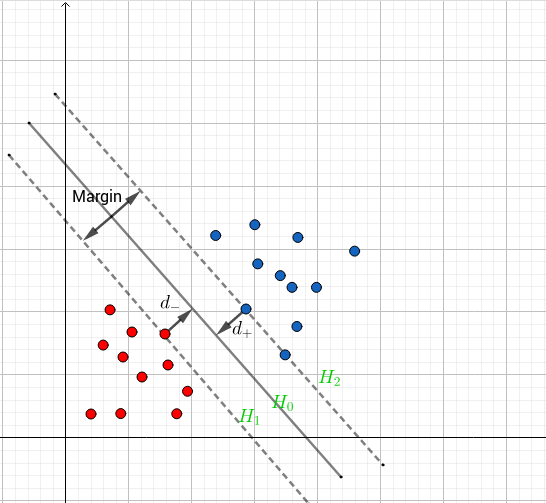
\includegraphics[width=0.75\linewidth]{images/svm.png}
		\caption{Support Vector Machine}
		\label{fig:writing-thesis}
	\end{figure}
	Và ta cần tính toán $w$ và $b$ để đưa ra quyết định về siêu phẳng tối ưu.
	\begin{gather*}
		w - \sum_{i=1}^m\alpha_iy_ix_i = 0\\
		\Leftrightarrow w = \sum_{i=1}^m\alpha_iy_ix_i
	\end{gather*}
	Để tính toán giá trị $b$
	\begin{gather*}
		y_i(w \cdot x^{*} + b) - 1 = 0\\
		\Leftrightarrow y_i^2(w \cdot x^{*} + b) - y_i = 0\\
		\Leftrightarrow b = y_i - w \cdot x^{*} 
	\end{gather*}
	Lưu ý: $y_i^2 = 1 \forall i$
	Và giá trị $b$ cũng có thể được tính
	\begin{gather*}
		b = \frac{1}{S}\sum_{i=1}^S(y_i - w \cdot x)
	\end{gather*}
	\textbf{Bước 04: Xây dựng hàm phân lớp từ những support vectors}\newline
	Bộ phân lớp được định nghĩa để đưa ra dự đoán. Hypothesis function h:
	\begin{gather*}
		h(x_i) = \begin{cases}+1, w \cdot x + b \geq 0\\ -1,  w \cdot x + b < 0\end{cases}
	\end{gather*}
	\textbf{Giải bài toán tối ưu SVM (SVM optimization problem) - Soft Margin SVM}\newline
	
	Bài toán Hard Margin SVM giải quyết tốt cho dữ liệu phân hoạch tuyến tính. Tuy nhiên, điều này dường như hiếm gặp trong thực tế. Hầu hết các trường hợp dữ liệu sẽ chứa nhiễu và có thể không phân hoạch tuyến tính (phân bố dạng cầu, ...)
	
	Soft Margin SVM sử dụng một trick rất đơn giản, thêm vào những biến chùng (slack variables) $\varsigma_i$ vào ràng buộc của bài toán tối ưu
	\begin{gather*}
		y_i(w \cdot x_i + b) \geq 1 - \varsigma_i, i =1...m
	\end{gather*}
	Nhờ sử dụng những biến chùng trong ràng buộc, khi cực tiểu hàm mục tiêu, nó có khả năng thõa mãn ràng buộc cho dù dữ liệu huấn luyện không thõa ràng buộc ban đầu. Và sử dụng L1 Regularization để giải quyết vấn đề của những giá trị biến chùng lớn. Ta có bài toán tối ưu như sau:
	\begin{gather*}
		\Leftrightarrow \underset{w, b}{\text{ min }}\frac{1}{2}||w||^2 + \sum_{i=1}^m\varsigma_i\\
		\text{subject to } y_i(w.x+b) \geq 1 - \varsigma_i, i = 1...m \\
	\end{gather*}
	Và để tránh việc phân lớp sai trong mỗi huấn luyện, ta thêm vào ràng buộc biến chùng không âm và tham số $C$ gọi là regularization parameter để xác định giá trị biến chùng $\varsigma$ quan trọng như thế nào?
	\begin{gather*}
		\Leftrightarrow \underset{w, b}{\text{ min }}\frac{1}{2}||w||^2 + C\sum_{i=1}^m\varsigma_i\\
		\text{subject to } y_i(w.x+b) \geq 1 - \varsigma_i, \varsigma_i \geq 0, i = 1...m \\
	\end{gather*}
	Và tiếp tục sử dụng nhân tử Lagrange, đưa bài toán về bài toán kép
	\begin{gather*}
		\underset{\alpha}{\text{ max }}\sum_{i=1}^m\alpha_i - \frac{1}{2}\sum_{i=1}^m\sum_{j=1}^m\alpha_i\alpha_j y_i y_j x_i \cdot x_j\\
		\text{subject to } 0 \leq \alpha_i \leq C, i = 1...m,  \sum_{i=1}^m\alpha_iy_i = 0\\
	\end{gather*}
	\subsubsection{b. Liệt kê một số nhân (kernel) phổ biến được sử dụng trong SVM}
	Một số nhân (kernel) phổ biết được sử dụng trong SVM như
	
	1) Linear kernel: $\mathbf{K}(\mathbf{x}_i, \mathbf{x}_j) = \mathbf{x}_i^T\mathbf{x}_j$ 
	
	2) Polynomial kernel: $\mathbf{K}(\mathbf{x}_i, \mathbf{x}_j) = (1 +  \mathbf{x}_i^T\mathbf{x}_j)^p$
	
	3) Gaussian (Radial-Basis Function (RBF) ) kernel:
	
	\begin{gather*}
		\mathbf{K}(\mathbf{x}_i, \mathbf{x}_j) = exp\left(-\frac{||\mathbf{x}_i - \mathbf{x}_j||^2}{2\sigma^2}\right)
	\end{gather*}
	
	4) Sigmoid:
	\begin{gather*}
		\mathbf{K}(\mathbf{x}_i, \mathbf{x}_j) = \text{tanh}(\beta_0\mathbf{x}_i^T\mathbf{x}_j + \beta_1)
	\end{gather*}
	
	
	\subsubsection{c. Phân biệt các chiến lược phân đa lớp: one vs. all và one vs. one}
	
	\begin{table}[H]
		\centering
		\begin{tabular}{| p{5cm} | p{5cm} | p{5cm} |}\hline
			& One vs one& One vs all \T\B\\\hline
		Ưu điểm & Dễ dàng sử dụng sau khi xử lí.
		Phù hợp khi bài toán có nhiều lớp. & Nhanh hơn khi hội tụ
		phù hợp khi bài toán có ít lớp.\T\B\\\hline
		Nhược điểm & Chậm hơn phân loại 2 lớp trong quá trình train. & Gần như không thể dùng khi có quá nhiều lớp.	\T\B\\\hline
		Phương pháp & Thuật toán sử dụng cây. Neural network. & SVM.
		Các phương pháp tập hợp.
		Thuật toán sử dụng cây.\T\B\\\hline
		\end{tabular}
	\end{table}
	
	\begin{figure}[H]
		\centering
		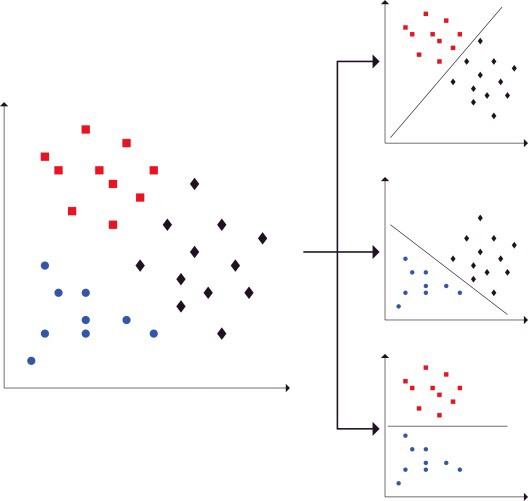
\includegraphics[width=0.75\linewidth]{images/one_vs_one.jpeg}
		\caption{Chiến lược one vs. one}
		\label{fig:writing-thesis}
	\end{figure}


	\begin{figure}[H]
		\centering
		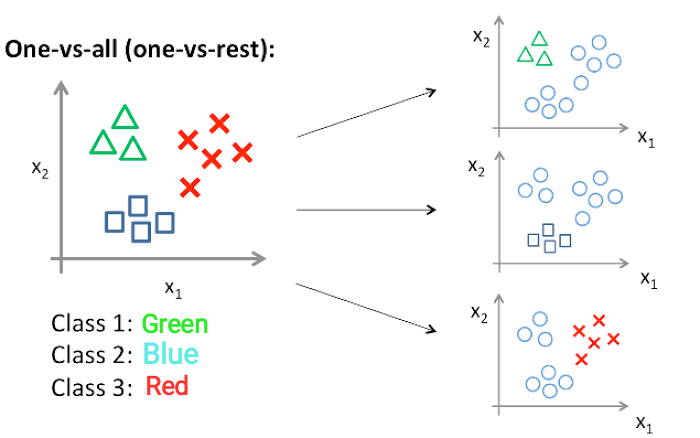
\includegraphics[width=0.75\linewidth]{images/one_vs_all.png}
		\caption{Chiến lược one vs. all}
		\label{fig:writing-thesis}
	\end{figure}
	
	\subsection{A.4 Kiến thức về mạng nơron cơ bản (ANN)}
	\qquad Cho trước một mạng neural với hai tầng: 
	- Tầng 1: nhận vào một ảnh nhập
	- Tầng 2 là tầng xuất ứng với 4 bộ phân lớp được xuất ra (Bộ phân lớp 1 đại diện cho 'học sinh nữ có tóc dài'; Bộ phân lớp 2 đại diện cho 'học sinh nam có tóc dài'; Bộ phân lớp 3 đại diện cho 'học sinh nữ có tóc ngẵn' và Bộ phân lớp 4 đại diện cho 'học sinh nam có tóc ngắn').
	
	Tuy nhiên, dữ liệu huấn luyện mạng phân bố không đều:
	- 4 mẫu cho bộ phân lớp 1
	- 4 mẫu cho bộ phân lớp 3
	- 4 mẫu cho bộ phân lớp 4
	- Riêng bộ phân lớp 2 chỉ có 1 mẫu huấn luyện
	
	Như vậy, bộ phân lớp 2 là yếu. Học viên hãy đề nghị một cấu trúc mạng nơ ron mới sao cho nâng hiệu quả bộ lớp 2 mà vẫn sử dụng bộ mẫu huấn luyện nói trên? Nêu lên tính hiệu quả của cấu trúc mạng nơ ron đề nghị?
	
	Đề nghị một cấu trúc mạng Neural tăng thêm một tầng cơ sở
	- Tầng 01: Tầng nhận ảnh đầu vào
	- Tầng 02 là tầng ẩn: Trong tầng này gồm hai bộ phân lớp
	- Bộ phân lớp 1 dùng để phân loại học sinh nam hay học sinh nữ gồm 8 mẫu huấn luyện cho nữ và 8 mẫu nam
	- Bộ phân lớp 2 dùng để phân loại tóc ngắn hay tóc dài gồm 5 mẫu huấn luyện tóc dài và 8 mẫu tóc ngắn
	- Tầng 03 là tập đầu ra với 4 bộ phân lớp: học sinh nữ có tóc dài, học sinh nam có tóc dài, học sinh nữ có tóc ngẵn, học sinh nam có tóc ngắn
	
	\begin{figure}[H]
		\centering
		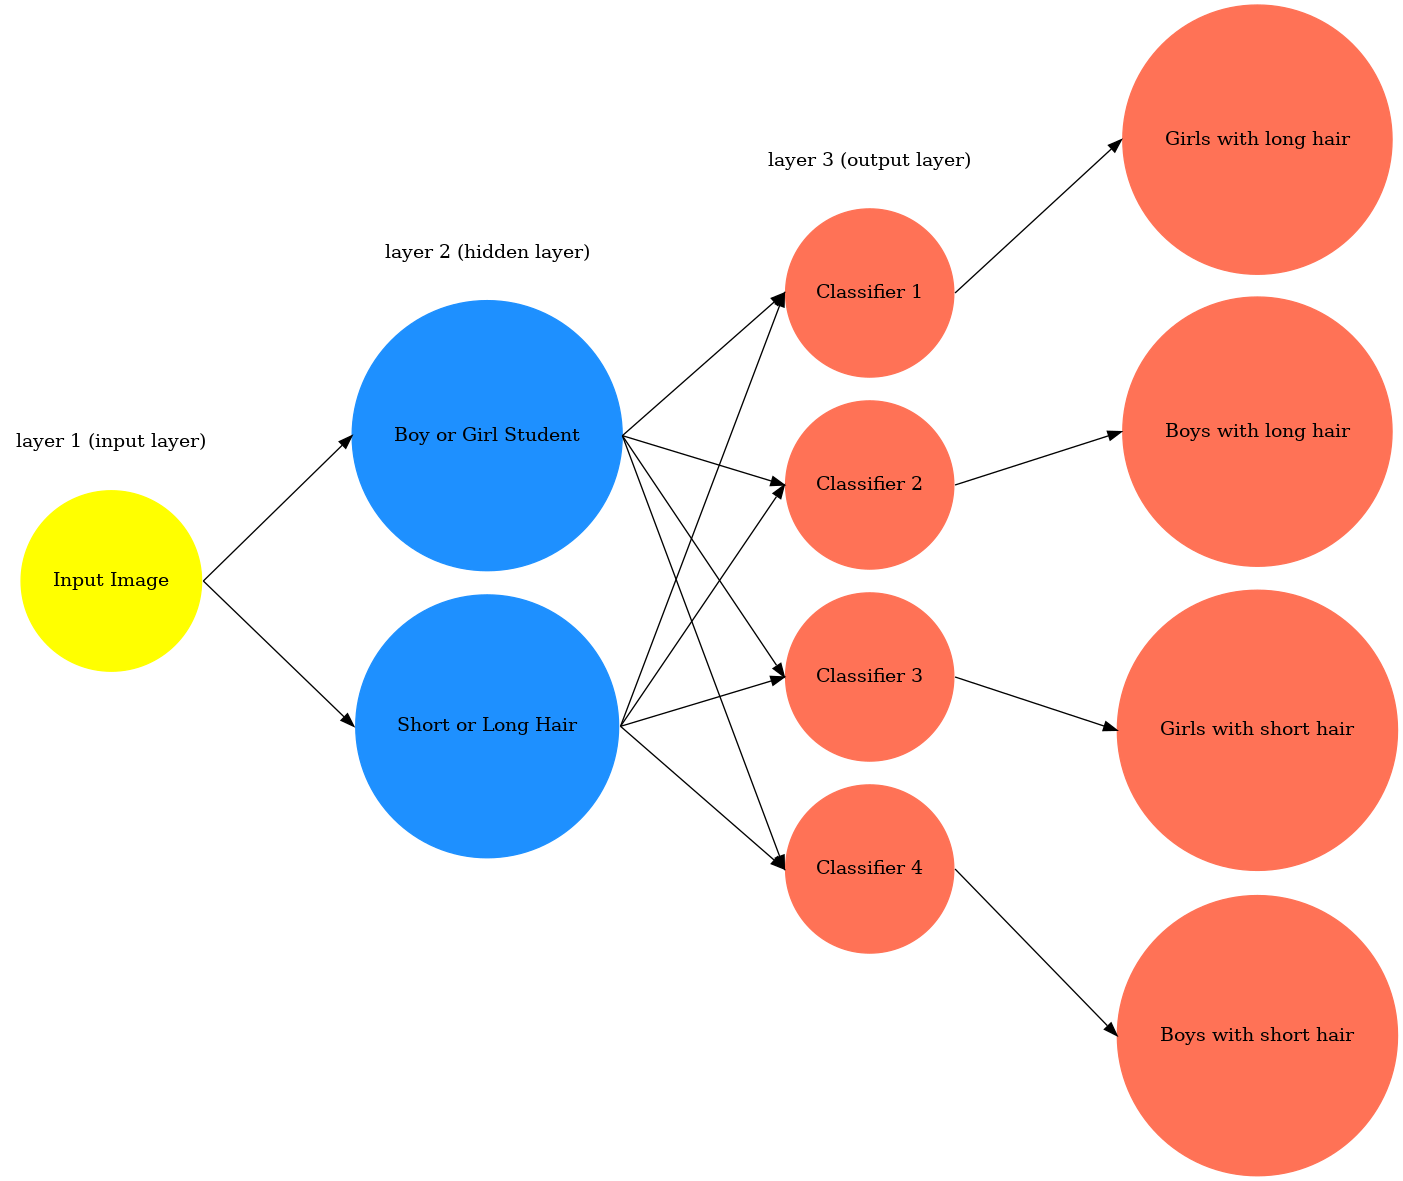
\includegraphics[width=0.75\linewidth]{images/nets.png}
		\caption{Kiến trúc mạng đề xuất}
		\label{fig:writing-thesis}
	\end{figure}
	
	Tính hiệu quả của cấu trúc mạng Neural:
	- Xây dựng thêm một tầng cơ sở với 2 bộ phân lớp, tăng cường dữ liệu cho mỗi bộ phân lớp, nên sẽ trả về kết quả tốt
	- Tầng phân lớp (tầng xuất) chỉ có nhiệm vụ tổng hợp các kết quả nhận được từ tầng cơ sở (không cần phải huấn luyện)
	
	
	\subsection{A.5 Kiến thức về mạng nơron sâu (DNN)}
	
	\subsubsection{a. Giải thích vì sau mạng nơron sâu thường cho kết quả tốt hơn mạng nơron rộng với cùng số
		lượng nơron.}
	
	\qquad Mạng neural rộng thường cần nhiều neural hơn để có thể thực hiện các tác vụ giống như mạng neural sâu: số lượng đơn vị trong một mạng neural rộng tăng lên theo cấp số nhân với độ phức tạp của nhiệm vụ. Vì vậy, để trở nên hữu ích, một mạng neural rộng có thể cần phải rất lớn; có thể lớn hơn nhiều so với một mạng sâu. Điều này dựa trên một số tài liệu chứng minh rằng các mạng neural rộng trong một số trường hợp cần nhiều nơ-ron theo cấp số nhân.
	
	Có thể một mạng neural rộng sẽ khó đào tạo hơn với các thuật toán hiện tại (ví dụ: khó xác định cực tiểu cục bộ hơn hoặc tốc độ hội tụ chậm hơn,…)
	
	Nhiều lớp thực hiện chung 1 tác vụ, hoặc có thể mỗi lớp xử lý một tác vụ khác nhau. Linh hoạt trong nhiều nhiệm vụ khác nhau.
	
	Kiến trúc của mạng neural rộng thường không phù hợp với các tác vụ hiện nay như nhận dạng, nhận diện.
	
	\begin{figure}[H]
		\centering
		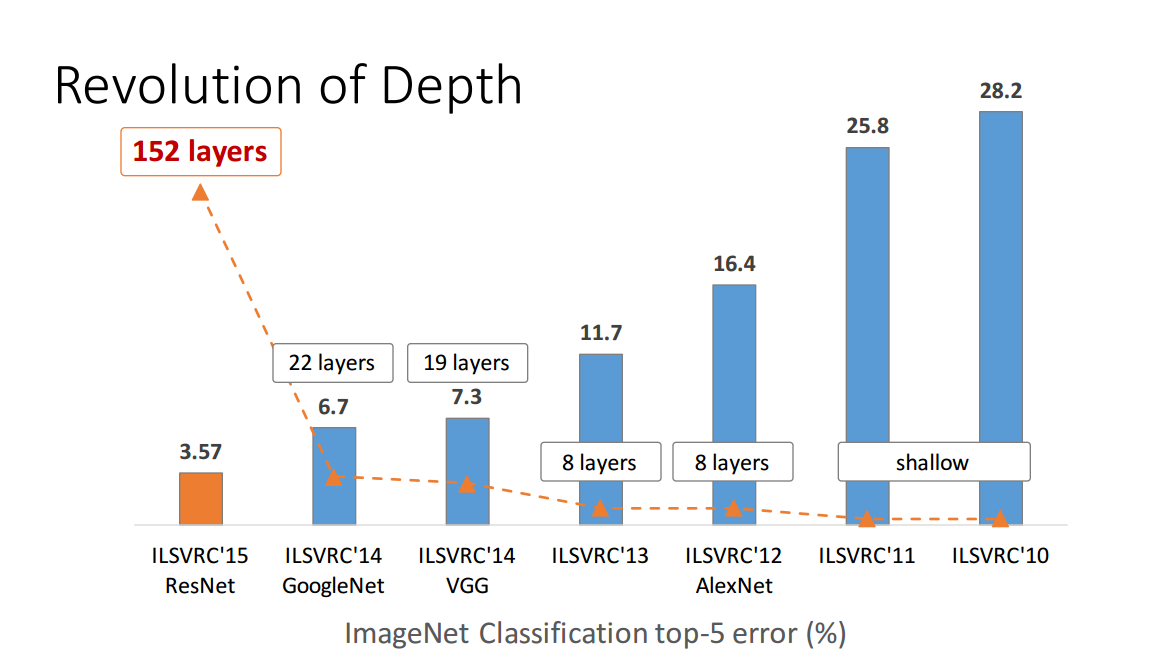
\includegraphics[width=1\linewidth]{images/a5_1.png}
		\caption{Revolution of Depth}
		\label{fig:writing-thesis}
	\end{figure}

	\begin{figure}[H]
		\centering
		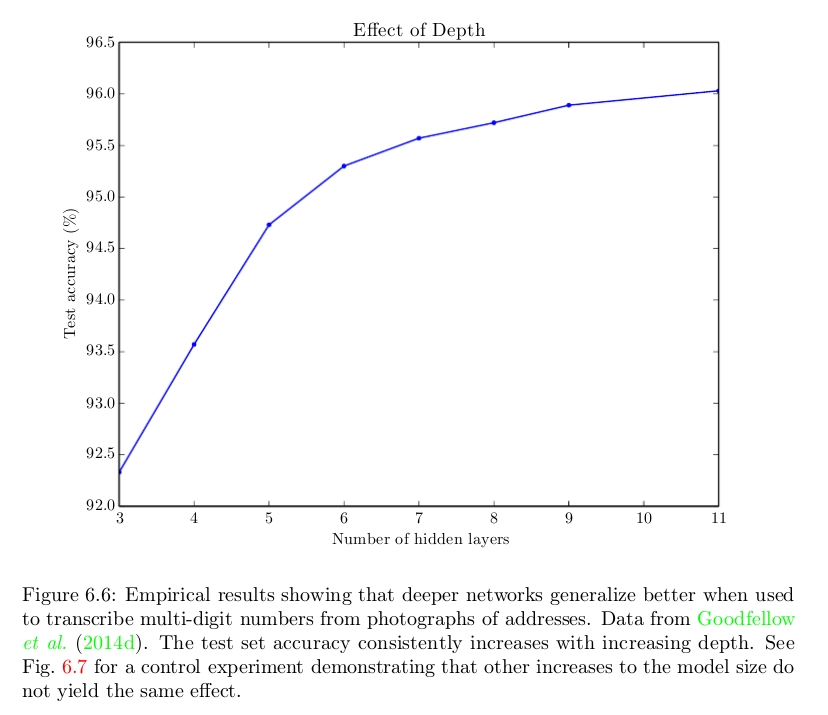
\includegraphics[width=1\linewidth]{images/a5_2.png}
		\caption{Revolution of Depth}
		\label{fig:writing-thesis}
	\end{figure}
	
	\subsubsection{b. Cho biết 3 dạng hàm kích hoạt (activation function) thường được sử dụng trong mạng sâu}
	\begin{figure}[H]
		\centering
		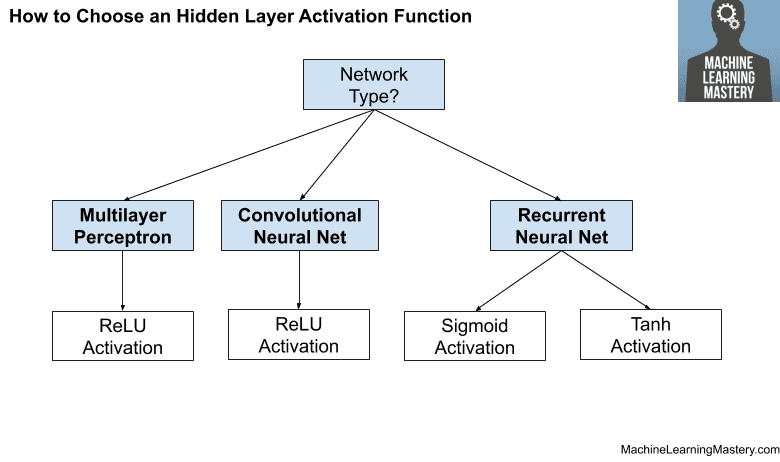
\includegraphics[width=1\linewidth]{images/a5_3.png}
		\caption{Revolution of Depth}
		\label{fig:writing-thesis}
	\end{figure}
	\textbf{Sigmoid function}\newline
	
	\begin{figure}[H]
		\centering
		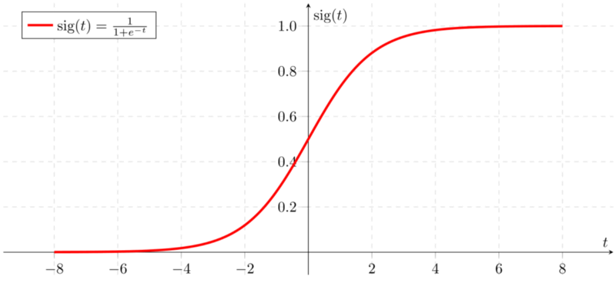
\includegraphics[width=0.75\linewidth]{images/a5_4.png}
		\caption{Trực quan hóa hàm Sigmoid Activation Function}
		\label{fig:writing-thesis}
	\end{figure}
	Biểu diễn toán học cho hàm như sau:
	$$S(x) = \frac{1}{1 + e^{-x}}$$
	
	Hàm kích hoạt tuyến tính tốt hơn trong việc cung cấp một loạt các kích hoạt và đường có độ dốc dương có thể làm tăng tốc độ bắn khi tốc độ đầu vào tăng.

	\begin{itemize}
		\item Ưu điểm: Đây là một loại hàm kích hoạt khá đơn giản và được sử dụng phổ biến vào những năm 1990.
		\item Khuyết điểm: độ bão hòa gradient, hội tụ chậm, gradient ẩm rõ nét(nguyên văn là sharp damp gradients) trong quá trình lan truyền ngược từ bên trong các lớp ẩn sâu hơn đến các lớp đầu vào, và đầu ra có điểm trung tâm khác 0 khiến các cập nhật gradient lan truyền theo các hướng khác nhau.
	\end{itemize}
	\textbf{Tanh function}\newline
	\begin{figure}[H]
		\centering
		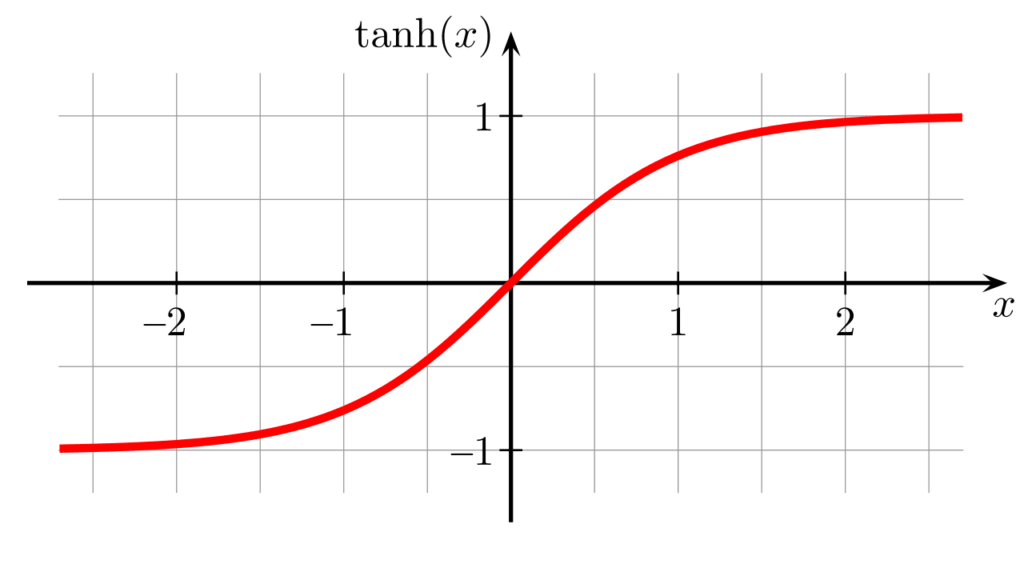
\includegraphics[width=0.75\linewidth]{images/a5_5.png}
		\caption{Trực quan hóa hàm Tanh Activation Function}
		\label{fig:writing-thesis}
	\end{figure}
	Biểu diễn toán học của hàm ReLU
	$$f(x) = \frac{e^x - e^{-x}}{e^x +  e^{-x}}$$
	Ưu điểm
	\begin{itemize}
		\item Hàm tanh được sử dụng rộng rãi hơn nhiều so với hàm sigmoid vì nó mang lại hiệu suất đào tạo tốt hơn cho các mạng nơ-ron đa lớp. Ưu điểm lớn nhất của hàm tanh là nó tạo ra đầu ra với điểm 0 là trung tâm, do đó hỗ trợ quá trình lan truyền ngược. Hàm tanh chủ yếu được sử dụng trong các mạng nơ-ron hồi quy cho các tác vụ xử lý ngôn ngữ tự nhiên và nhận dạng giọng nói.
	\end{itemize}
	Nhược điểm
	\begin{itemize}
		\item Hàm tanh cũng có một hạn chế - giống như hàm sigmoid, nó không thể giải quyết vấn đề gradient biến mất. Ngoài ra, hàm tanh chỉ có thể đạt được độ dốc bằng 1 khi giá trị đầu vào là 0 (x bằng 0). Kết quả là, hàm có thể tạo ra một số tế bào thần kinh chết trong quá trình tính toán.
	\end{itemize}
	\textbf{ReLU Activation Function}\newline
	\begin{figure}[H]
		\centering
		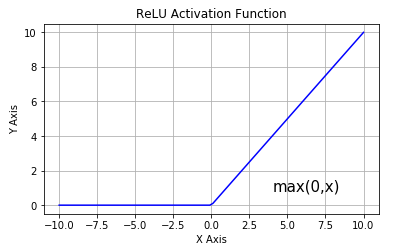
\includegraphics[width=0.75\linewidth]{images/relu_activation_function.png}
		\caption{Trực quan hóa hàm ReLU Activation Function}
		\label{fig:writing-thesis}
	\end{figure}
	Biểu diễn toán học của hàm ReLU
	$$f(x) = max(0, x)$$
	
	Ưu điểm của ReLU:
	\begin{itemize}
		\item Bằng cách ràng buộc các giá trị của đầu vào nhỏ hơn 0 và đặt chúng thành 0, và ngưỡng tối đa của hàm này ở vô cực - loại bỏ vấn đề gradient biến mất được quan sát trong các loại hàm kích hoạt trước đó (sigmoid và tanh). Ưu điểm đáng kể nhất của việc sử dụng hàm ReLU trong tính toán là nó đảm bảo tính toán nhanh hơn - nó không tính toán theo cấp số nhân và phép chia, do đó thúc đẩy tốc độ tính toán tổng thể. Một khía cạnh quan trọng khác của hàm ReLU là nó tạo ra sự thưa thớt trong các đơn vị ẩn bằng cách bình phương các giá trị từ 0 đến lớn nhất.
	\end{itemize}
	Nhược điểm của ReLU:
	\begin{itemize}
		\item ReLU có thể chết trong quá trình huấn luyện, nơi chúng ngừng học hoàn toàn, vì vậy chúng ta cần phải cẩn thận về phạm vi giá trị đầu vào.
	\end{itemize}
	\begin{figure}[H]
		\centering
		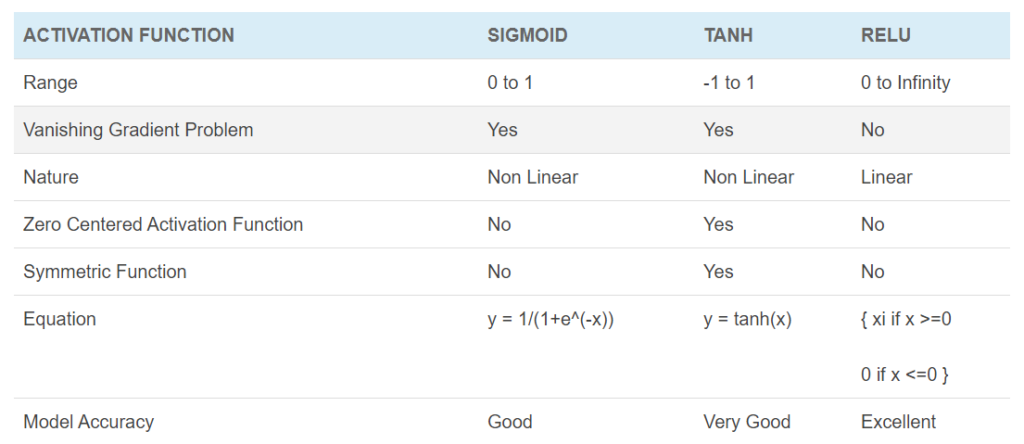
\includegraphics[width=0.75\linewidth]{images/a5_6.png}
		\label{fig:writing-thesis}
	\end{figure}
	\subsubsection{c. Cho biết 3 bộ tối ưu hóa (optimizer) thường được sử dụng trong mạng sâu}
	\qquad Mục tiêu chính của học máy là tạo ra một mô hình hoạt động tốt và đưa ra các dự đoán chính xác trong một số trường hợp cụ thể. Để đạt được điều đó, chúng ta cần tối ưu hóa học máy. Tối ưu hóa học máy là quá trình điều chỉnh các siêu tham số để giảm thiểu hàm chi phí bằng cách sử dụng một trong các kỹ thuật tối ưu hóa. Điều quan trọng là phải giảm thiểu hàm chi phí vì nó mô tả sự khác biệt giữa giá trị thực của thông số ước tính và những gì mô hình đã dự đoán.
	
	\textbf{1) Batch normalization}
	
	\textbf{Ý tưởng cơ bản:} Chuẩn hóa là một kỹ thuật để thay đổi giá trị của các cột số trong tập dữ liệu thành một tỷ lệ chung mà không làm sai lệch sự khác biệt trong phạm vi giá trị. Kỹ thuật này thường được áp dụng như một phần của quá trình chuẩn bị dữ liệu cho học máy và cần thiết nếu các đặc trưng đầu vào khác nhau nằm trong một phạm vi giá trị khác nhau.
	
	\textbf{Ưu điểm}
	\begin{itemize}
		\item Mạng huấn luyện nhanh hơn - Mỗi lần lặp lại việc huấn luyện sẽ chậm hơn do các tính toán bổ sung trong quá trình chuyển tiếp và các siêu tham số bổ sung để huấn luyện trong quá trình lan truyền ngược. Tuy nhiên, nó sẽ hội tụ nhanh hơn nhiều, vì vậy việc huấn luyện tổng thể trở nên nhanh hơn. 
		\item Cho phép tỷ lệ học tập cao hơn - Giảm dần độ dốc thường yêu cầu tốc độ học tập nhỏ để dễ hội tụ. Và đối với mạng học sâu, độ dốc của chúng sẽ nhỏ dần trong quá trình lan truyền ngược, vì vậy chúng đòi hỏi nhiều lần lặp lại hơn. Sử dụng chuẩn hóa hàng loạt cho phép người dùng sử dụng tốc độ học tập cao hơn nhiều, điều này làm tăng thêm tốc độ huấn luyện mạng. 
		\item Làm cho trọng số khởi tạo dễ dàng hơn - Khởi tạo trọng số có thể khó và càng khó hơn khi tạo các mạng học sâu. Chuẩn hóa hàng loạt dường như cho phép chúng ta bớt cẩn thận hơn trong việc chọn trọng số ban đầu.
		\item Làm cho nhiều hàm kích hoạt khả thi hơn - Một số hàm kích hoạt không hoạt động tốt trong một số trường hợp. Sigmoid mất gradient khá nhanh, có nghĩa là chúng không thể được sử dụng trong các mạng sâu. Và ReLU thường chết trong quá trình huấn luyện, nơi chúng ngừng học hoàn toàn, vì vậy chúng ta cần phải cẩn thận về phạm vi giá trị đầu vào. Chuẩn hóa hàng loạt, điều chỉnh các giá trị đi vào mỗi hàm kích hoạt, các yếu tố phi tuyến tính dường như không hoạt động tốt trong các mạng học sâu giờ đây đã có thể hoạt động tốt trở lại.
		\item Đơn giản hóa việc tạo các mạng học sâu - Do 4 ưu điểm được liệt kê ở trên.
		\item Có thể cho kết quả tổng quát tốt hơn - Một số thử nghiệm dường như cho thấy quá trình chuẩn hóa hàng loạt thực sự cải thiện kết quả huấn luyện.
	\end{itemize}

	\textbf{Nhược điểm}
	\begin{itemize}
		\item Khó ước tính giá trị trung bình và độ lệch chuẩn của đầu vào trong quá trình kiểm tra.
		\item Không thể sử dụng kích thước batch là 1 trong quá trình huấn luyện.
		\item Chi phí tính toán trong quá trình huấn luyện khá cao. bước chuyển tiếp lịch sử được mang theo mỗi bước, và những đi những bước lớn thì không phải lúc nào cũng tốt
		\item Cách tính khác nhau giữa việc huấn luyện và kiểm tra không phù hợp cho Mạng Neural Hồi quy (Recurrent Neural Network) và Mạng bộ nhớ ngắn hạn dài (Long Short-Term Memory Network)
	\end{itemize}
	
	\textbf{2) Mini-batch gradient descent}Là một biến thể của thuật toán gradient descent chia các tập dữ liệu huấn luyện thành các nhóm nhỏ được sử dụng để tính toán lỗi mô hình và cập nhật hệ số mô hình.
	
	\textbf{Ưu điểm}
	\begin{itemize}
		\item Tần suất cập nhật mô hình cao hơn so với Batch gradient descent.
		\item Kiểm soát dữ liệu huấn luyện trong bộ nhớ tốt hơn giúp cho qua trình triển khai thuật toán hoạt động trơn tru.
		\item Cập nhật liên tục, cung cấp một quy trình tính toán hiệu quả hơn so với Stochastic gradient descent.
	\end{itemize}
	\textbf{Nhược điểm}
		\begin{itemize}
		\item Không đảm bảo sự hội tụ của một lỗi theo cách tốt hơn.
		\item Vì 50 mẫu dữ liệu được lấy, không đại diện cho các thuộc tính (hoặc phương sai) của toàn bộ tập dữ liệu. Do đó, đây là lý do mà chúng ta sẽ không thể có được sự hội tụ, tức là chúng ta sẽ không nhận được cực tiểu cục bộ hoặc toàn cục tại bất kỳ thời điểm nào.
		\item Khi sử dụng Mini-batch gradient descent, vì các mẫu được lấy theo từng nhóm, do đó, có thể xảy ra trường hợp trong một số nhóm xuất hiện lỗi này, một số lại xuất hiện lỗi khác. Vì vậy, chúng ta sẽ phải tự mình kiểm soát tốc độ học tập, bất cứ khi nào chúng ta sử dụng Mini-Batch gradient descent. Nếu tỷ lệ học tập rất thấp, tỷ lệ hội tụ cũng sẽ giảm. Nếu tỷ lệ học tập quá cao, ta sẽ không nhận được mức cực tiểu cục bộ hoặc toàn cục. Vì vậy chúng ta cần kiểm soát tốc độ học.
	\end{itemize}

	\textbf{3) RMSProp optimization} RMSprop là một kỹ thuật tối ưu hóa dựa trên gradient. Nó được đề xuất bởi cha đẻ của lan truyền ngược, Geoffrey Hinton. Gradient của các hàm phức tạp như mạng nơ-ron có xu hướng biến mất khi dữ liệu truyền qua các hàm đó. RMSprop được phát triển như một kỹ thuật ngẫu nhiên để học theo từng nhóm nhỏ.
	
	RMSprop giải quyết vấn đề trên bằng cách sử dụng đường trung bình động của các bình phương gradient để chuẩn hóa gradient. Quá trình chuẩn hóa này cân bằng kích thước ở mỗi bước (bước nhảy), giảm bước cho các gradient lớn để tránh sự đột ngột tăng lên và tăng bước cho các gradient nhỏ để tránh biến mất. 
	
	\textbf{Ưu điểm}
	\begin{itemize}
		\item RMSProp hội tụ nhanh, trong nhiều cài đặt. Đặc biệt là đối với GAN, RL và mạng dựa trên sự chú ý. RMSProp có thể hội tụ các giải pháp với chất lượng tốt hơn (ví dụ: cực tiểu cục bộ tốt hơn). Ít biến thiên so với các thuật toán như Gradient Descent.
	\end{itemize}
	\textbf{Nhược điểm}
	\begin{itemize}
		\item Tỷ lệ học tập vẫn phải cài đặt thủ công, vì giá trị đề xuất không phải lúc nào cũng phù hợp cho mọi tác vụ. Triển khai RMSProp Descent cần có sự giám sát.
	\end{itemize}
	
	\subsubsection{d. Trình bày kỹ thuật Dropout}
	\qquad Thuật ngữ "Dropout" đề cập đến việc bỏ qua các đơn vị (units) ẩn và hiện trong 1 mạng Neural.
	
	Hiểu 1 cách đơn giản thì Dropout là việc bỏ qua các đơn vị (tức là 1 nút mạng) trong quá trình huấn luyện 1 cách ngẫu nhiên. Bằng việc bỏ qua này thì đơn vị đó sẽ không được xem xét trong quá trình lan truyền và lan truyền ngược.
	
	Theo đó, $p$ được gọi là xác suất giữ lại 1 nút mạng trong mỗi giai đoạn huấn luyện, vì thế xác suất nó bị loại bỏ là $(1 – p)$.
	\begin{figure}[H]
		\centering
		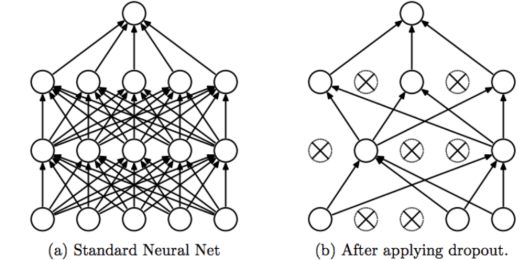
\includegraphics[width=0.75\linewidth]{images/a5_7.png}
		\label{fig:writing-thesis}
	\end{figure}
	Công dụng: Làm đơn giản mô hình, tránh overfitting. Thêm vào đó, vì mỗi bước khi train model thì xác suất (1-p) các node bị loại bỏ nên model không thể phụ thuộc vào bất kì node nào của layer trước mà thay vào đó có xu hướng trải đều weights. 
	
	Một số tips: Hệ số $p$ nên ở khoảng $[0.2, 0.5]$ . Nếu p quá nhỏ thì không có tác dụng chống overfitting, tuy nhiên nếu $p$ quá lớn thì gần như loại bỏ layer đấy và có dễ dẫn đến underfitting. Nên dùng model lớn, phức tạp hơn vì ta có dropout chống overfitting. Dropout chỉ nên dùng cho fully connected layer, ít khi được dùng cho ConvNet layer. Hệ số $p$ ở các layer nên tỉ lệ với số lượng node trong FC layer đó.
	
	Kỹ thuật này được sử dụng như sau:
	\begin{itemize}
		\item Trong pha train: với mỗi hidden layer, với mỗi trainning sample, với mỗi lần lặp, chọn ngẫu nhiên p phần trăm số node và bỏ qua nó (bỏ qua luôn hàm kích hoạt cho các node bị bỏ qua).
		\item Trong pha test: Sử dụng toàn bộ activations, nhưng giảm chúng với tỷ lệ $p$ (do chúng ta bị miss $p\%$ hàm activation trong quá trình train).
	\end{itemize}
	
	\section{B. Bài tập thực tế}
	
	
	\subsection{B.1 Mạng Neural Tích Chập và bài toán Nhận Dạng}
	
	\subsubsection{a) Mô tả tổng quan về mạng nơron tích chập (CNN)}
	\qquad Những công trình đầu tiên vào năm 1959 của David Hubel và Torsten Wiesel đưa ra mô tả về "\textbf{simple cell}" và "\textbf{complex cell}" trong vỏ não thị giác của con người (human visual cortex) và được đề xuất sử dụng trong lĩnh vực Nhận dạng mẫu (Pattern Recognition)
	
	 Một "Simple cell" tương ứng với cạnh và đường trục trong một không gian cụ thể:
	\begin{figure}[H]
		\centering
		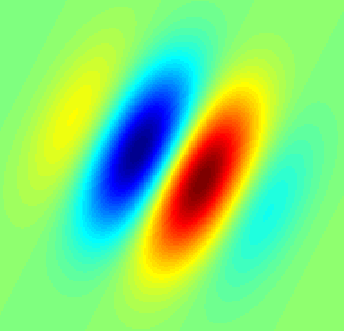
\includegraphics[width=0.5\linewidth]{images/simple_cell.png}
		\caption{Simple Cell}
		\label{fig:writing-thesis}
	\end{figure}
	Một "Complex cell" cũng tương ứng với cạnh và đường trục trong một không gian cụ thể nhưng nó khá khác so với "Simple cell"
	\begin{figure}[H]
		\centering
		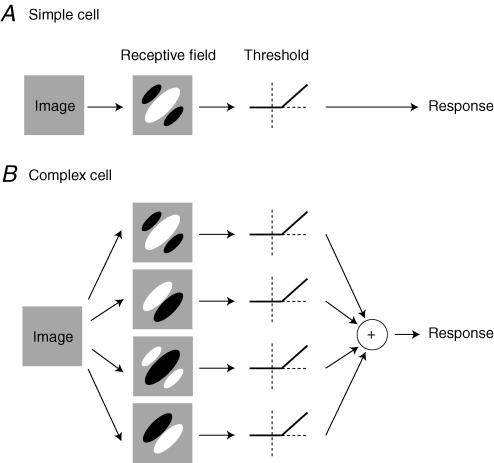
\includegraphics[width=0.5\linewidth]{images/complex_cell_simple_cell.jpg}
		\caption{Simple Cell}
		\label{fig:writing-thesis}
	\end{figure}
	Với "simple cell" có thể chỉ ứng với một trục ngang ở cạnh dưới của một bức ảnh, còn với "complex cell" có thể ứng các trục ngang ở dưới (bottom), giữa (middle) hoặc trên cùng (top) của một bức ảnh.
	
	Cho đến năm 1962, Hubel và Wiesel đề xuất một công trình cho thấy rằng Complex Cell đạt được bất biến không gian bằng cách "\textbf{summing}" - tổng hợp đầu ra của nhiều simple cell tham chiếu cùng hướng (cùng đường trục) nhưng khác nhau về vị trí tiếp nhận (có thể bottom, middle hoặc top). Khái niệm về một bộ nhận diện phức tạp có thể được tổng hợp từ nhiều bộ nhận diện đơn giản được phát hiện trong \textbf{hệ thống thị giác con người (human visual system)} và trở thành khái niệm cơ sở cho những \textbf{mô hình Convolution Neural Networks}.
	
	Trong những năm 1980, Dr. Kunihiko Fukushima dựa trên ý tưởng công trình Simple cell và Complex cell của Hubel và Wiesel, đề xuất mô hình tên là "\textbf{neocognition}" trong bài báo "\textbf{Neocognitron: A Self-organizing Neural Network Model for a Mechanism of Pattern Recognition Unaffected by Shift in Position}”. Mô hình bao gồm hai thuật ngữ quan trọng "S-cells" và "C-cells" định nghĩa toán tử toán tử. S-cells được đặt ở tầng đầu tiên của mô hình và được liên kết với C-cell nằm ở tầng hai của mô hình. Nhờ vào đây, người ta có thể biến nó thành mô hình tính toán cho Nhận dạng mẫu thị giác (Visual Pattern Recognition) với ý tưởng "\textbf{simple-to-complex}".
	
	Công trình đầu tiên đặt nền móng cho Convolution Neural Network hiện đai xuất hiện vào những năm 1990, bởi Giáo sư Yann LeCun và đồng nghiệp công bố trong bài báo của họ "\textbf{Gradient-Based Learning Applied to Document Recognition}”, và đến nay đã có hơn 38019 lượt citation cho bài báo này. Xuất phát từ ý tưởng của mô hình neocognition, công trình của giáo sư trình bày một mô hình CNN tổng hợp những đặc trưng đơn vào những đặc trưng phức tạp hơn có thể được sử dụng cho nhận dạng chữ viết tay (handwritten character recognition)
	
	Một cách tổng quát, hầu hết các phương pháp dựa trên Neural Networks thường là những phương pháp có giám sát (supervised methods). Không chỉ các bài toán dự đoán hồi quy (regression) hay bài toán phân lớp (classification), nhưng có thể là không giám sát, do đó, tùy vào yêu cầu bài toán, với bài toán phân loại, chúng ta cần dữ liệu huấn luyện được gán nhãn trước, quá trình huấn luyện là giám sát, nhưng với bài toán gom cụ, ví dụ như gom cụm hình ảnh dựa trên độ tương đồng, thì các Neural Network đóng vai trò như bộ rút trích và được kết hợp với một số phương pháp không giám sát như K-means, ... 
	
	Với Convolution Neural Networks được sử dụng khá rộng rãi trong hầu hết các bài toán như phân lớp hình ảnh (Image Classification), nhận dạng vật thể (Object Recognition), các bài toán nhận dạng sinh trắc học (Biometric Recognition) như Nhận dạng khôn mặt, Nhận dạng vân tay, Nhận dạng dáng đi, Nhận dạng mẫu mắt, ... ngay cả Nhận dạng giọng nói/ người nói, nó chỉ dùng trong giai đoạn rút trích đặc trưng từ bức ảnh, tổng hợp và chồng chéo các khu vực nhỏ trên bức ảnh.

	\subsubsection{b) Các bài toán nhận dạng có thể được giải quyết bằng mạng nơron tích chập (CNN)}
	\qquad Một số bài toán nhận dạng có thể được giải quyết bằng mạng  nơron tích chập (CNN)\newline
	\textbf{Bài toán 1: Nhận dạng vân tay dựa trên CNN}\newline
	1) \textbf{Phát biểu bài toán}\newline
	\begin{itemize}
		\item Đầu vào: Hình ảnh vân tay
		\item Đầu ra: Lớp của vân tay
	\end{itemize}
	2) \textbf{Phương pháp thực hiện}\newline
	Minh họa phương pháp được sử dụng ở \cite{sym13050750}
	\begin{figure}[H]
		\centering
		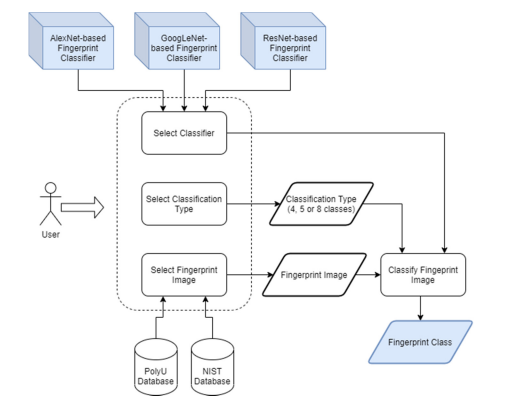
\includegraphics[width=0.75\linewidth]{images/finger_recognition.png}
		\caption{Hệ thống nhận dạng vân tay}
		\label{fig:writing-thesis}
	\end{figure}
	CNNs đóng vai trò như bộ phân lớp, dựa trên mạng học đã được huấn luyện từ trước với rất nhiều tham số như AlexNet, GoogleNet, ResNet.
	
	\textbf{Bài toán 2:  Nhận dạng khuôn mặt dựa trên CNN}\newline
	1) \textbf{Phát biểu bài toán}\newline
	\begin{itemize}
		\item Đầu vào: Dữ liệu hình ảnh khuôn mặt
		\item Đầu ra: Lớp của hình ảnh khuôn mặt
	\end{itemize}
	2) \textbf{Phương pháp thực hiện}\newline
	\begin{figure}[H]
		\centering
		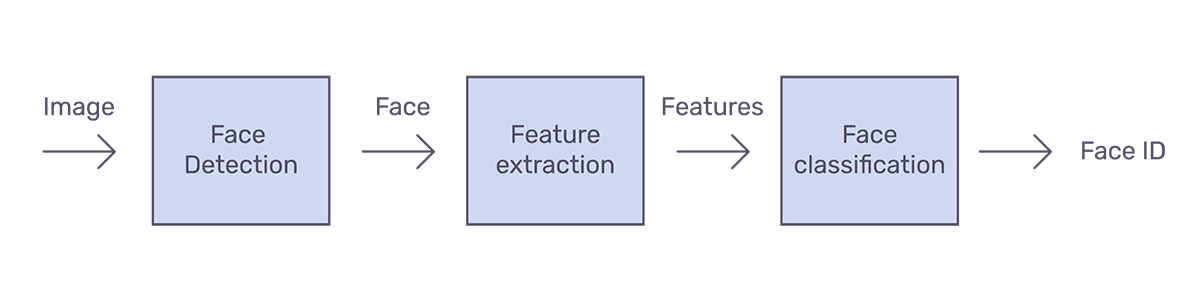
\includegraphics[width=0.75\linewidth]{images/face-recognition-pipeline.png}
		\caption{Hệ thống nhận dạng khuôn mặt}
		\label{fig:writing-thesis}
	\end{figure}
	\begin{itemize}
		\item Face detection: Nhận diện một hay nhiều khuôn mặt trong một bức ảnh
		\item Feature extraction: Rút trích đặc trưng quan trọng từ một bức ảnh khuôn mặt
		\item Face classification: Phân lớp khuôn mặt dựa trên những đặc trưng được rút trích
	\end{itemize}
	Tham khảo từ: https://arsfutura.com/magazine/face-recognition-with-facenet-and-mtcnn/
	
	Face Recognition Framework bao gồm những thành phần như MTCNN cho face detection, FaceNet cho việc phát sinh face embedding và dùng Softmax như một bộ phân lớp.
	
	Dùng FaceNet để học:
	\begin{itemize}
		\item Chọn ngẫu nhiễn một anchor image
		\item Chọm ngẫu nhiên một ảnh cùng một người với ảnh anchor
		\item Chọn ngẫu nhiên một ảnh khác người với ảnh anchor
		\item Hiệu chỉnh tham số FaceNet để ảnh với ảnh anchor hơn là ảnh khác với anchor
	\end{itemize}
	
	\textbf{Bài toán 3: Nhận dạng người nói dựa trên CNN}\newline
	1) \textbf{Phát biểu bài toán}\newline
	
	Bài toán nhận dạng người nói thường được chia thành hai tác vụ con, gồm: xác minh người nói (speaker verification) và định danh người nói (speaker identification). Xét bài toán con xác minh người nói (speaker verification)
	\begin{itemize}
		\item Đầu vào: dữ liệu âm thanh giọng nói
		\item Đầu ra: Đồng ý (Accept)/ Từ chối (Deny)
	\end{itemize}
	2) \textbf{Phương pháp thực hiện}\newline
	Minh họa phương pháp được sử dụng ở \cite{Alzubaidi2021ReviewOD}
		
	Trong giai đoạn phát triển (development stage), lời nói của các người nói được sử dụng để tạo ra một mô hình nền cho việc đại diện người nói. Sử dụng kiến trúc DNN như một bộ rút trích đặc trưng người nói mạnh mẽ.
	
	Trong giai đoạn đăng ký (Enrollment stage), một mô hình phân biệt sẽ được tạo cho mỗi định danh người nói. Những lời nói của người nói sẽ được sử dụng để phát sinh mô hình người nói. Trong DNN, lời nói của người nói sẽ là đầu vào của mô hình được tạo ra ở giai đoạn trước đó, và đầu ra được tích hợp với một số phương pháp để cho ra một mô hình người nói.
	
	Trong giai đoạn đánh giá (Evaluation stage), những lời nói kiểm gia sẽ được đưa vào bộ rút trích đại diện người nói, truy vấn kiểm tra mẫu sẽ được so sánh với tất cả mô hình người nói bằng cách sử dụng một hàm tính điểm (score function) nào đó và điểm cao nhất được chọn là người nói được dự đó của mô hình.
	
	CNN đóng vai trò như một bộ rút trích đặc trưng từ dữ liệu đầu vào, là những sóng âm thanh thô, được tinh chỉnh và dùng kỹ thuật cửa sổ (ví dụ hamming windows) trong miền tần số, làm CNN có thể hoạt động tương tự như xử lý với ảnh số.
	
	\subsubsection{c) Mô tả tư tưởng chủ đạo và các bước chính trong giải thuật của mạng nơron tích chập (CNN)}
	
	Mạng neural Tích Chập (hay được biết là Convolutional Neural Networks - CNNs) được hình thành từ ba ý tưởng chính:
	\begin{itemize}
		\item Tiếp nhận khu vực cục bộ (local receptive fields)
		\item Chia sẻ trọng số (Shared weights)
		\item Tổng hợp (Pooling)
	\end{itemize}

	Hai tính chất đặc trưng của CNNs:
	\begin{itemize}
		\item Những mẫu (patterns) mà CNNs học là bất biến với phép tịnh tiến
		\item CNNs có thể học những chiều phân cấp của mẫu
	\end{itemize}
	Kiến trúc cơ bản của CNN
	\begin{figure}[H]
		\centering
		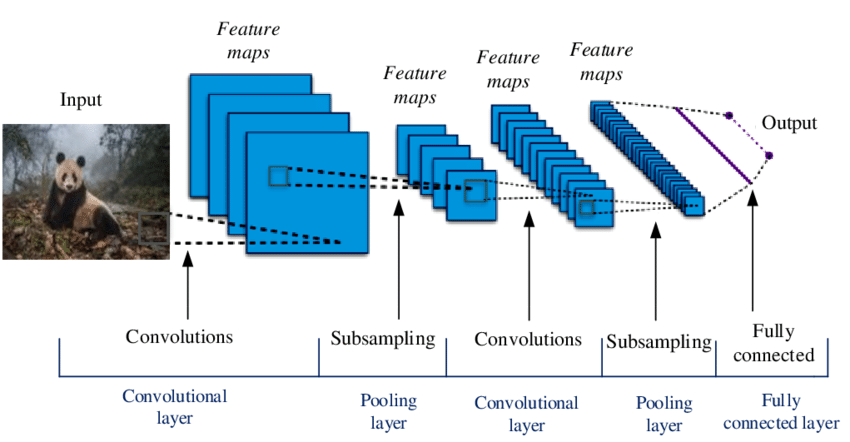
\includegraphics[width=0.75\linewidth]{images/An-example-of-a-simple-CNN-architecture.png}
		\caption{Kiến trúc cơ bản mạng CNNs}
		\label{fig:writing-thesis}
	\end{figure}
	\textbf{Lớp Convolutional - Convolutional Layer}
	Trong Xử lý ảnh số và Video số (Digital Image and Video Processing), một bức ảnh đầu vào được tích chập với một nhân (kernel) để tạo ra một ảnh đầu ra (output image)\newline
	\begin{itemize}
		\item Input Image (Input feature map)
		\item Output Image (Output feature map)
		\item Filter (Bộ lọc) gồm ba tham số:
		\begin{itemize}
			\item Kích thước nhân (kernel) F cho biết phạm vi không gian của kernel
			\item Stride S cho biết khoảng cách giữa hai vị trí liên tiếp nhau của nhân (kernel)
			\item Số lượng bộ đệm không (zero padding) P cho biết dố lượng các số không được thêm vào từ vị trí bắt đầu đến vị trí kết thúc của một trục
		\end{itemize}
	\end{itemize}
	Ta có thể sử dụng hai toán tử cho việc tính tích chập gồm Convolution Operator và Cross-correlation operator
	\begin{itemize}
		\item Toán tử Convolution được sử dụng nhiều trong Xử lý ảnh số
		\begin{equation}
			\text{Output}(x, y) = (K * \text{Input})(x, y) = \sum_m\sum_n\text{Input}(x-m, y-m)K(m,n)
		\end{equation}
		\item Toán tử Cross-correlation được sử dụng trong mạng CNN
		\begin{equation}
			\text{Output}(x, y) = (K * \text{Input})(x, y) = \sum_m\sum_n\text{Input}(x+m, y+m)K(m,n)
		\end{equation}
	\end{itemize}
	Ví dụ:
	
	Ảnh đầu vào (Input image) có kích thước $7 \times 7$
	
	Ảnh đầu ra (Output image) có kích thước $5 \times 5$
	
	Nhân (Kernel) có kích thước $F = 3$, $S = 1$, $P = 0$
		
	\begin{center}
	\convoutionpicture 14
	\bigskip
	
	\convoutionpicture 41
	\bigskip
	
	\convoutionpicture 55
	\end{center}

	\textbf{Lớp tổng hợp - Pooling layer} nhiệm vụ chính của lớp này là sub-sampling các feature map, tác nó thành những feature map nhỏ hơn
	
	\begin{tikzpicture}
		\fill [c1] (0, 0) rectangle (2, 2);
		\fill [c2]   (2, 0) rectangle (4, 2);
		\fill [c3]  (4, 0) rectangle (6, 2);
		\fill [c4] (0, 2) rectangle (2, 4);
		\fill [c5]   (2, 2) rectangle (4, 4);
		\fill [c6]   (4, 2) rectangle (6, 4);
		
		\fill [c1]  (9.5, 1) rectangle (10.5, 2);
		\fill [c2]   (10.5, 1) rectangle (11.5, 2);
		\fill [c3]  (11.5, 1) rectangle (12.5, 2);
		\fill [c4]  (9.5, 2) rectangle (10.5, 3);
		\fill [c5]   (10.5, 2) rectangle (11.5, 3);
		\fill [c6]   (11.5, 2) rectangle (12.5, 3);
		
		\foreach \i in {\xMin,...,\xMax} {
			\draw [very thin,gray] (\i,\yMin) -- (\i,\yMax)  node [below] at (\i,\yMin) {};
		}
		\foreach \i in {\yMin,...,\yMax} {
			\draw [very thin,gray] (\xMin,\i) -- (\xMax,\i) node [left] at (\xMin,\i) {};
		}
		
		\foreach \i in {\xMin,2,...,\xMax} {
			\draw [thick,gray] (\i,\yMin) -- (\i,\yMax)  node [below] at (\i,\yMin) {};
		}
		\foreach \i in {\yMin,2,...,\yMax} {
			\draw [thick,gray] (\xMin,\i) -- (\xMax,\i) node [left] at (\xMin,\i) {};
		}
		\node at (0.5, 0.5) {7};
		\node at (1.5, 0.5) {9};
		\node at (2.5, 0.5) {3};
		\node at (3.5, 0.5) {5};
		\node at (4.5, 0.5) {9};
		\node at (5.5, 0.5) {4};
		%
		\node at (0.5, 1.5) {0};
		\node at (1.5, 1.5) {7};
		\node at (2.5, 1.5) {0};
		\node at (3.5, 1.5) {0};
		\node at (4.5, 1.5) {9};
		\node at (5.5, 1.5) {0};
		%
		\node at (0.5, 2.5) {5};
		\node at (1.5, 2.5) {0};
		\node at (2.5, 2.5) {9};
		\node at (3.5, 2.5) {3};
		\node at (4.5, 2.5) {7};
		\node at (5.5, 2.5) {5};
		%
		\node at (0.5, 3.5) {9};
		\node at (1.5, 3.5) {2};
		\node at (2.5, 3.5) {9};
		\node at (3.5, 3.5) {6};
		\node at (4.5, 3.5) {4};
		\node at (5.5, 3.5) {3};
		
		\draw[draw=black,line width=12pt,-{Latex[length=9mm]}] (6.5, 2)  -- (9,2);
		\node[font=\footnotesize\bfseries] at (7.7, 2.5) {$\mathbf{2\times 2}$ max pooling};
		
		\foreach \i in {\xMinR,...,\xMaxR} {
			\draw [thick,gray] (\i,\yMinR) -- (\i,\yMaxR)  node [below] at (\i,\yMinR) {};
		}
		\foreach \i in {\yMinR,...,\yMaxR} {
			\draw [thick,gray] (\xMinR,\i) -- (\xMaxR,\i) node [left] at (\xMinR,\i) {};
		}
		
		\node at (10, 1.5) {9};
		\node at (11, 1.5) {5};
		\node at (12, 1.5) {9};
		\node at (10, 2.5) {9};
		\node at (11, 2.5) {9};
		\node at (12, 2.5) {7};
		
		\draw [decorate,decoration={brace,amplitude=4pt},xshift=-2pt,yshift=0pt]
		(0,2) -- (0,4) node [black,midway,xshift=-0.3cm] {\footnotesize $2$};
		
		\draw [decorate,decoration={brace,amplitude=4pt},xshift=0pt,yshift=2pt]
		(0,4) -- (2,4) node [black,midway,yshift=+0.3cm] {\footnotesize $2$};
	\end{tikzpicture}

	\textbf{Activation Function (non-linearity)} ánh xạ đầu vào thành đầu ra, được coi là hàm cốt lõi (core function) của tất cả các hàm kích hoạt của tất cả các loại mạng Neural. Một hàm kích hoạt thường gặp như: Sigmoid, Tanh, ReLU, Leaky ReLU, Noisy ReLU, Parametric Linear Units

	\textbf{Lớp Fully-Connected Layers}
	Fully connected layers còn được gọi là affine layers, tạo ra suy luận mức cao (high-level reasoning) trong DNN. Những neuron trong một fully connected layer kết nối đầy đủ với tất cả các kích hoạt trong layer trước đó.
	
	\begin{figure}[H]
		\centering
		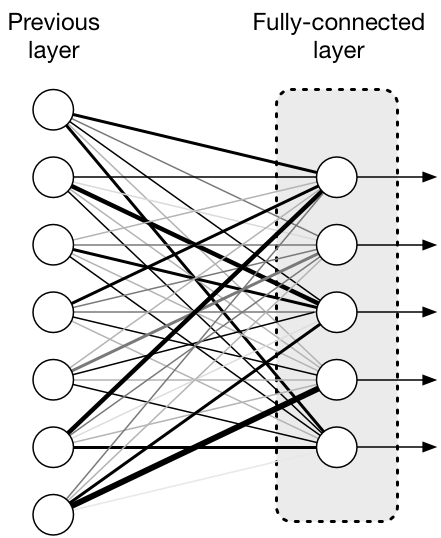
\includegraphics[width=0.5\linewidth]{images/FullyConnectedLayer.png}
		\caption{Kiến trúc cơ bản mạng CNNs}
		\label{fig:writing-thesis}
	\end{figure}

	\textbf{Loss Function - Hàm mất mát} là những hàm dùng để tính toán độ lỗi trong quá trình huấn luyện, nó tính toán độ lỗi giữa giá trị đúng (actual values) với giá trị dự đoán (predicted values) để tối ưu việc học trong mạng CNN. Một số hàm mất mát thường gặp như: Cross-Entropy hay Softmax Loss Function, Euclidean Loss Function, Hinge Loss Function
	
	\subsubsection{d) Đánh giá ưu điểm và khuyết điểm của mạng nơron tích chập (CNN) về nhiều phương diện}
	Ưu điểm của mạng nơron tích chập (CNN)
	\begin{itemize}
		\item CNN chia sẻ trọng số đặc trưng, mà làm giảm số lượng tham số huấn luyến có thể có và nó giúp mạng học tăng cường phát sinh và tránh overfitting
		\item Những tầng rút trích đặc trưng (feature extraction layers) và tầng phân lớp (classifcation layer) học một cách đồng thời vì đầu ra của mô hình vừa được tổ chức cao vừa có độ tin cậy cao vào các tính năng được trích xuất.
		\item Cài đặt mạng ở mức độ quy mô một cách dễ dàng với CNN hơn những mạng Neural khác.
	\end{itemize}
	Nhược điểm
	\begin{itemize}
		\item Cần nhiều sức mạnh tính toán, ví dụ như sử dụng GPU, TPU hay các máy chủ có cấu hình mạnh
		\item Hiệu năng phụ thuộc vào dữ liệu đầu vào, liệu nó có sạch hay không, có đủ nhiều hay không, có cân bằng hay không
		\item Quá nặng, việc nhúng vào các phần cứng bị hạn chế tài nguyên là một thách thức lớn.
	\end{itemize}
	
	\subsection{B.2 YOLOX: Cải thiện YOLO ( You Only Look Once)}
	
	\subsubsection{a) Mô tả tổng quan về giải pháp nhận dạng được chọn}

	\qquad Với mục đích cải thiện YOLO, YOLOX là một thuật toán có khả năng phát hiện và xác minh các loại vật, người trong hình ảnh, từ đó xác minh trong video. Xác minh vật trong YOLO được thực hiện như 1 bài toán hồi quy và cung cấp xác suất phân lớp vật trong hình được dùng.
	
	Thuật toán YOLO sử dụng CNN để xác minh vật theo thời gian thực. thuật toán này chỉ yêu cầu 1 lần lan tỏa trên mạng network để phát hiện vật. 

	Việc dự đoán vật trên hình chỉ qua 1 lần xử lí giúp cho YOLO trở thành 1 trong những thuật toán xử lí real-time tốt nhất hiện nay. 

	YOLO được phát triển qua thời gian với nhiều biến thể khác, YOLOX là 1 trong những biến thể đó.
	
	Cá nhân/ tổ chức đang phát triển YOLO: Joseph Redmon, người đầu tiên và chính thức phát triển YOLO.
	
	Cá nhân/ tập thể sử dụng tiềm năng:
	\begin{itemize}
		\item Chính phủ sử dụng cho quản lí về đường bộ.
		\item Các công ty bất kì để kiểm soát công viên làm việc.
		\item Camera giám sát trong những tòa nhà ở hay những cá nhân sử dụng bảo vệ căn nhà.
	\end{itemize}
	Tài liệu tham khảo đến bài báo:
	\begin{itemize}
		\item YOLO: \href{https://www.section.io/engineering-education/introduction-to-yolo-algorithm-for-object-detection/}{https://www.section.io/engineering-education/introduction-to-yolo-algorithm-for-object-detection/}
		\item Link bài báo YOLO: \href{https://arxiv.org/abs/1506.02640}{https://arxiv.org/abs/1506.02640}
		\item YOLOX: \href{https://arxiv.org/abs/2107.08430}{https://arxiv.org/abs/2107.08430}
		\item Paper with code: \href{https://paperswithcode.com/paper/yolox-exceeding-yolo-series-in-2021}{https://paperswithcode.com/paper/yolox-exceeding-yolo-series-in-2021}
		\item YOLO v5: \href{http://www.xfkj.com.cn/EN/abstract/abstract510.shtml}{http://www.xfkj.com.cn/EN/abstract/abstract510.shtml}
		\item Code: \href{https://github.com/Megvii-BaseDetection/YOLOX}{https://github.com/Megvii-BaseDetection/YOLOX}
		\item Trang chủ của Joseph Redmon: \href{https://pjreddie.com/}{https://pjreddie.com/}
	\end{itemize}
	
	\subsubsection{b) Liệt kê các tính năng chủ đạo của giải pháp}
	\begin{itemize}
		\item Tốc độ xử lí ảnh: thuật toán này cải thiện tốc độ phát hiện vật bởi nó có khả năng và sử dụng trong hệ thống thời gian thực.
		\item Độ chính xác cao: YOLO là 1 kĩ thuật dự đoán cho ra kết quả xác suất chính xác cao với tỉ lệ sai thấp.
		\item Khả năng học: thuật toán có khả năng học hoàn hảo cho phép nó học đại diện vật và áp dụng xác minh các vật tương đương.
	\end{itemize}
	Tài liệu tham khảo:
	\begin{itemize}
		\item https://arxiv.org/pdf/2107.08430.pdf ( YOLOX)
		\item https://www.section.io/engineering-education/introduction-to-yolo-algorithm-for-object-detection/ (YOLO)
		\item https://arxiv.org/ftp/arxiv/papers/2012/2012.07630.pdf (decoupled head) 
		\item \href{https://openaccess.thecvf.com/content\_CVPR\_2020/papers/Zhang\_Bridging\_the\_Gap\_Between\_Anchor-Based\_and\_Anchor-Free\_Detection\_via\_Adaptive\_CVPR\_2020\_paper.pdf}{https://openaccess.thecvf.com/content\_CVPR\_2020/papers/Zhang\_Bridging\_the\_Gap\_Between\_Anchor-Based\_and\_Anchor-Free\_Detection\_via\_Adaptive\_CVPR\_2020\_paper.pdf} (Anchor-free)
	\end{itemize}
	Thuật toán trong YOLO: \newline
	\textbf{Residual blocks}:
	\begin{itemize}
		\item Bức ảnh được quét sẽ chia thành nhiều ô nhỏ, mạng lưới này có không gian từng lưới là S x S. như được thể hiện qua hình dưới đây.
		\begin{figure}[H]
			\centering
			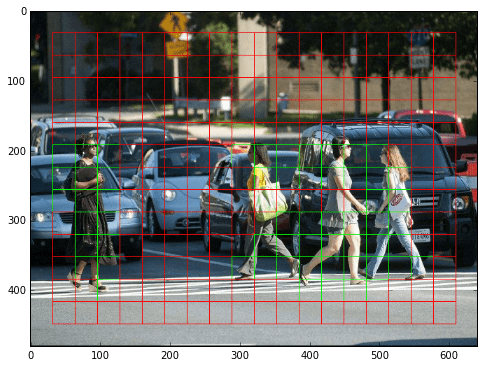
\includegraphics[width=1\linewidth]{images/b2_1.png}
			\label{fig:writing-thesis}
		\end{figure}
		Từ đó , xác minh đối tượng trên từng khung S x S. nhóm ô sẽ được cố định để tìm vật, qua đó xác minh danh tính của nhóm ô.
	\end{itemize}
	\textbf{Bounding box regression}:
	\begin{itemize}
		\item Các ô sau khi được nối liền sẽ trở thành 1 khối ô với đặc tính nhất định.
		\begin{itemize}
			\item Độ rộng.
			\item Độ cao
			\item Lớp.
			\item Tọa độ tâm.
		\end{itemize}
		Khối ô sẽ được qua xử lí hồi quy để dự đoán các số liệu trên, từ đó xác định được vật ( lớp).
	\end{itemize}
	\textbf{Intersection over union (IOU)}:\newline
	IOU là một hiện tượng xảy ra khi các ô ở lưới bị overlap. YOLO sử dụng IOU để tạo ra 1 box ảo, box ảo này được tạo ra với mục đích làm cho việc dự đoán vật trong mỗi ô nhỏ trở nên dễ dàng hơn. 

	Kết hợp 3 phương pháp lại với nhau.
	\begin{figure}[H]
			\centering
			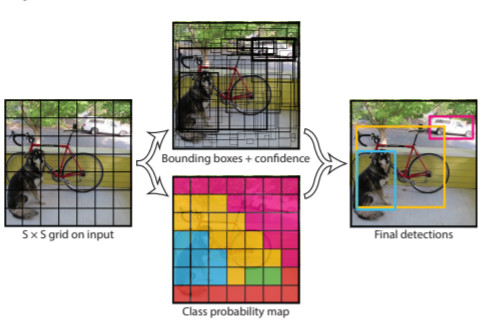
\includegraphics[width=1\linewidth]{images/b2_2.png}
			\label{fig:writing-thesis}
	\end{figure}
	Đầu tiên ảnh được chia thành 1 lưới những ô S x S. trên mỗi ô đó thực hiện bounding box và dự đoán class của vật, với tỉ lệ chính xác được đặt trên từng ô. Tiếp theo, nhờ vào IOU, những ô này sẽ được quyết định tỉ lệ của vật khi cắt bỏ hoặc thêm vào những grid thiếu/ thừa bởi IOU. Giảm thiểu những ô thừa sẽ tăng tỉ lệ dự đoán chính xác cho vật cần xác minh.
	
	Qua demo của bản thân và kết quả :
	\begin{figure}[H]
			\centering
			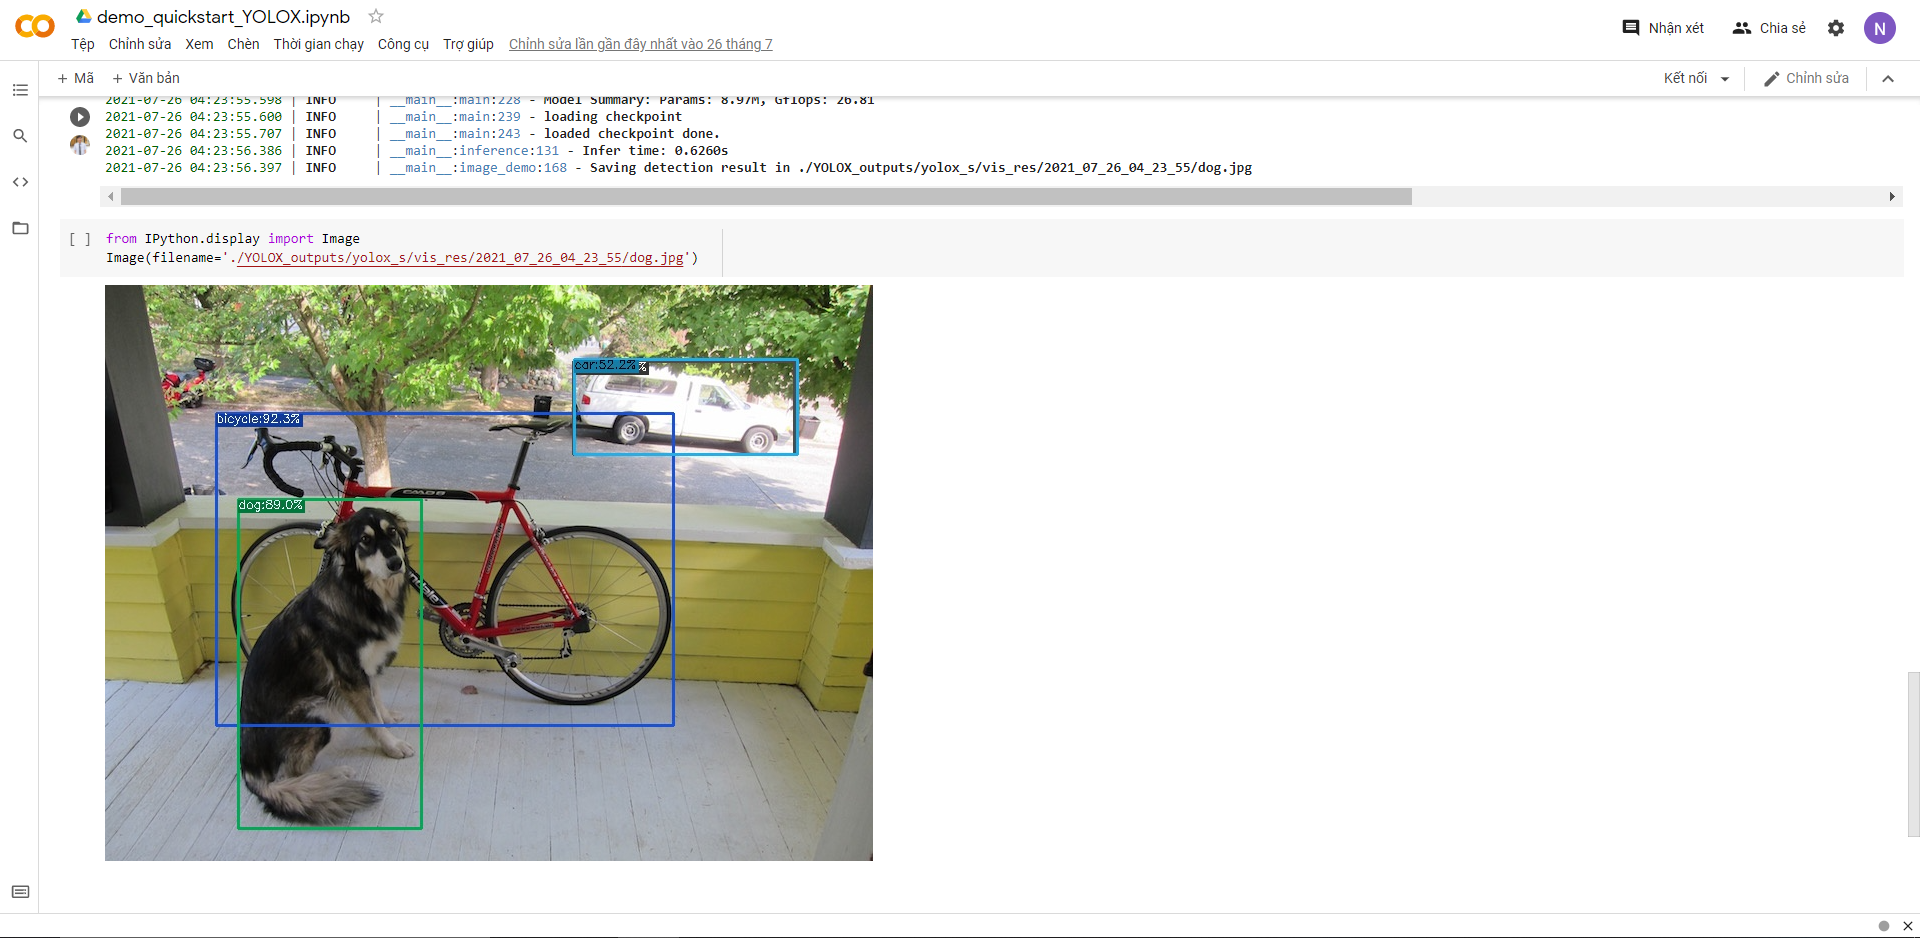
\includegraphics[width=1\linewidth]{images/b2_3.png}
			\label{fig:writing-thesis}
	\end{figure}
	
	Việc dự đoán phụ thuộc vào nhiều yếu tố như: độ sáng của ảnh, tỉ lệ độ lớn vật trong khung hình hay kết cấu trên vật tạo ra grid.

	YOLOX được phát triển từ YOLOv3 với công cụ Darknet53. YOLOX có các thay đổi so với YOLO về số liệu là chủ yếu, thay đổi về learning rate, IOU loss, BCE loss, …
	Sử dụng decouple head hay vì couple head bởi:
	\begin{itemize}
		\item Thay thế decouple head vào YOLO làm cho tốc độ hội tụ khi training được tăng lên đáng kể.
		\item Decoupled head là cần thiết đối với phiên bản YOLO.
	\end{itemize}
	\begin{figure}[H]
			\centering
			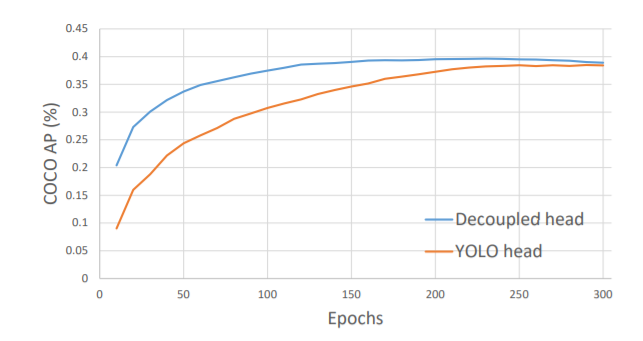
\includegraphics[width=1\linewidth]{images/b2_4.png}
			\label{fig:writing-thesis}
	\end{figure}
	Sử dụng Anchor-free thay cho Anchor-based:
	Anchor-free xác định các điểm keypoints cố định và nới rộng vật theo các keypoint đó.

	Hoặc xác định các ô cấu tạo vật, và bám theo điểm trung tâm của khối vật đó.

	Thay vì sử dụng anchor based và trải qua nhiều bước để xử lí được vật xác minh, anchor-free thể hiện tương tác cao hơn và tốc độ xử lí  nhanh hơn, là điều cần nhắm đến khi sử dụng trong ứng dụng real-time.
	\subsubsection{c) Đánh giá ưu điểm và khuyết điểm của giải pháp}
	\qquad YOLOX tập trung vào việc cải thiện thời gian xử lí để phù hợp với việc thực hiện real-time video. Bỏ qua các yếu tố như, độ chính xác, xử lí hình ảnh, xác định khu vực vật.
	
	Những ưu điểm:
	\begin{itemize}
		\item Có độ chính xác tương đối cao, tốc độ xử lí hoàn hảo để sử dụng cho real-time video. 
		\item Được phát triển với nhiều phiên bản phù hợp với yêu cầu đa dạng của người dùng.
		\item Là thuật toán mới được phát triển gần đây, sử dụng những phương pháp khá mới.
		\item Sẽ tiếp tục được phát triển nhiều hơn ở tương lai cũng như hiện tại, bởi sự đa dạng về phiên bản cũng như các bước thực hiện.
	\end{itemize}
	Những khuyết điểm:
	\begin{itemize}
		\item Độ chính xác không được tốt, chưa thực sự hoàn hảo
	\end{itemize}
	\subsubsection{d) Nhận diện ít nhất hai giải pháp khác}
	Một số giải pháp khác
	
	\textbf{R-CNN, Faster R-CNN, Mask R-CNN}:
	
	Được phát triển bởi các nhà nghiên cứu làm việc tại Google, các phương pháp sử dụng CNN được phát triển đầu tiên và đang ngày càng được cải thiện qua từng ngày.

	Input sẽ được đưa vào và cắt các mảnh được xem là vật cần xác định. Thực hiện lặp lại để ra được vật nhỏ trong vật lớn, từ đó đảm bảo được lấy được khung hình vừa vặn nhất so với vật cần tìm, và đảm bảo tính đúng đắn đối với các vật có trong hình.

	Tương tự như YOLO, CNN cũng được phát triển qua nhiều phiên bản theo từng năm, với phiên bản mới nhất hiện nay là Mask R-CNN.

	\textbf{CenterNet}:
	
	Sử dụng keypoint để xác định điểm tâm, từ đó giãn ô và xác định vật.

	Bằng cách xem như vật chỉ là 1 điểm tâm, bộ dự đoán sử dụng keypoint để để xác định được tính chất của vật, vị trí trên mô hình 3D, định hướng vật, hay dáng của vật.

	CenterNet là phương pháp khác biệt, đơn giản hơn, nhanh hơn, và chính xác hơn so với việc sử dụng lưới hay chia ô. 

	CenterNet đạt được khả năng đánh đổi tốc độ-độ chính xác cao nhất trên dataset COCO.  Với khả năng thực hiện real-time. Đây là 1 thuật toán khá tương đồng với YOLO.
	\subsection{B.3 Sử dụng CNN và RNN cho một bài toán nhận dạng} \qquad Trình bày một bài toán mà tồn tại cả giải pháp sử dụng CNN (hoặc biến thể của nó) và giải pháp sử dụng RNN (hoặc biến thể của nó)
	
	\subsubsection{a) Phát biểu bài toán}
	
	\qquad Bài toán: Nhận dạng giọng nói
	
	Giới thiệu: Trong nhận dạng giọng nói hay nhận dạng chữ viết tay, đầu ra sẽ là một câu, nhưng chưa hoàn chỉnh vì có các ký tự lặp lại như "heelllo", "toooo", ... hay các chữ có những khoảng trống (blank) như "he l l oo", "t o o", ... . Nguyên nhân dẫn tới những hiện tượng này là giọng nói dài (các đoạn ngân nga trong các bài hát, ...), giọng bị ngắt quãng, kích thước chữ viết tay lớn, nhỏ, ...
	
	Do đó, để cho ra được một câu hoàn chỉnh thì ta cần phải căn chỉnh lại đầu ra ấy, loại bỏ các ký tự lặp lại và khoảng trống.
	
	Bài toán này có nhiều ứng dụng thực tế như trợ giúp cho người khuyết tật về thị giác, tự động hóa, giáo dục,….
	
	\textbf{Input}: Dữ liệu âm thanh giọng nói thô.
	
	\textbf{Output}: Đưa ra chuỗi ký tự được nói chính xác.
	
	\subsubsection{b) Mô tả tổng quan về giải pháp nhận dạng sử dụng mạng nơron tích chập (CNN)}
	
	\begin{figure}[H]
		\centering
		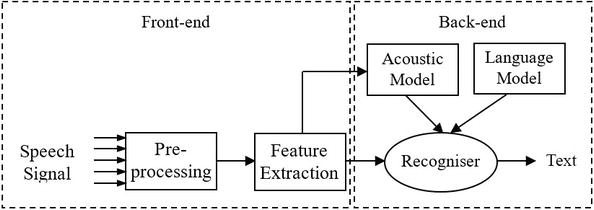
\includegraphics[width=1\linewidth]{images/b3_1.png}
		\caption{General framework of automatic speech recognition system}
		\label{fig:writing-thesis}
	\end{figure}

	\qquad Mạng nơ ron tích chập hay convolutional neural network (CNN) là mạng dạng tiếp thuận (feedforward) trong đó thông tin chỉ đi theo một chiều từ đầu vào đến đầu ra. CNN là một deep neural network (DNN). Hiểu đơn giản, nó cũng chính là một dạng artificial neural network (ANN), một multi-layer perceptron (MLP) nhưng mang thêm 1 vài cải tiến, đó là convolution và pooling. Gồm một lớp đầu vào, các lớp ẩn và một lớp đầu ra. Các lớp ẩn thực hiện việc tích chập đầu vào mỗi lớp và đưa ra đầu ra, tương ứng với đầu vào của các lớp tiếp theo. Mỗi lớp tích chập được mô tả có ba trạng thái : tích chập, tổng hợp và phi tuyến tính.
	
	CNN sử dụng các hàm phi tuyến để xử lý trực tiếp dữ liệu mức thấp. CNN có khả năng học các tính năng cấp cao với độ phức tạp và trừu tượng cao. 
	
	Pooling là phần quan trọng nhất của CNN giúp giảm kích thước của bản đồ đặc trưng. Pooling là một khái niệm biến biểu diễn đặc điểm chung thành thông tin có giá trị bằng cách giữ lại thông tin hữu ích và loại bỏ thông tin không quan trọng. Sự thay đổi tần số nhỏ thường gặp trong tín hiệu giọng nói được xử lý hiệu quả bằng cách sử dụng Pooling. Việc Pooling chung cũng giúp giảm phương sai phổ có trong lời nói đầu vào. Nó ánh xạ đầu vào từ p đơn vị liền kề thành đầu ra bằng cách áp dụng một hàm đặc biệt. Sau khi dùng hàm phi tuyến lên các phần tử chứa nhiều thông tin, các đặc trưng được chuyển qua lớp Pooling. Lớp này thực hiện việc lấy mẫu xuống trên các bản đồ đối tượng đến từ lớp trước và tạo ra các bản đồ đối tượng mới cô đọng. Lớp này làm giảm đáng kể kích thước và chiều của input. Nó phục vụ hai mục đích chính. Đầu tiên là giảm gần 65\% kích thước của input, giảm chi phí tính toán. Ngoại ra, lớp này còn kiểm soát việc xảy ra overfitting.
	
	\begin{figure}[H]
		\centering
		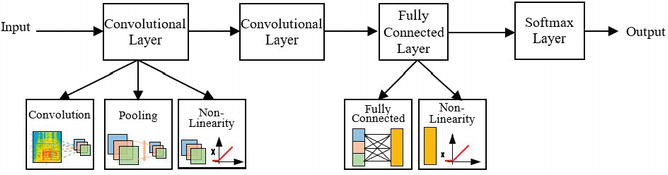
\includegraphics[width=1\linewidth]{images/b3_2.png}
		\caption{CNN Architecture}
		\label{fig:writing-thesis}
	\end{figure} 

	CNN-based raw speech phoneme recognition system là một mô hình được để xuất bởi Palaz. Trong đó tín hiệu giọng nói thô đầu vào sẽ được chia thành các tín hiệu giọng nói đầu vào. 
	
	\begin{gather*}
		s_t^c = \{s_{t-c}, ..., s_t, s_{t+c}\}
	\end{gather*}
	
	\begin{figure}[H]
		\centering
		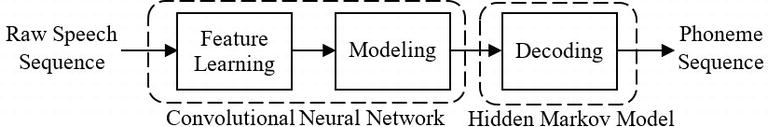
\includegraphics[width=1\linewidth]{images/b3_3.png}
		\caption{CNN-based raw speech phoneme recognition systeme}
		\label{fig:writing-thesis}
	\end{figure} 

	Tương ứng với 2c frame, mỗi frame có cửa sổ kéo dài trong $w_{in}$ milliseconds. Lớp tích chập đầu tiên học các đặc trưng có ích trong tín hiệu giọng nói thô. Các lớp tích chập còn lại thực hiện nhiệm vụ tiếp tục xử lý các đặc trưng thành thông tin có ích. 
	
	Sau khi xử lý tín hiệu giọng nói, CNN đánh giá xác suất có điều kiện của từng lớp  Một số giai đoạn lọc có trong mạng trước giai đoạn phân loại. Giai đoạn lọc là sự kết hợp của lớp chập, lớp gộp và lớp phi tuyến. Việc huấn luyện chung của giai đoạn rút trích đặc trưng và giai đoạn phân loại được thực hiện bằng cách sử dụng thuật toán lan truyền ngược.
	
	Cách tiếp cận của phương pháp này được mô tả như sau: Tín hiệu lời nói có bản chất là không cố định. Do đó, chúng được xử lý theo phương thức ngắn hạn. Các phương pháp trích xuất đặc trưng truyền thống thường sử dụng kích thước cửa sổ xử lý 20–40 ms. Trong phương pháp này, việc xử lý tín hiệu trong thời gian ngắn là bắt buộc. Do đó, kích thước của cửa sổ xử lý được coi là siêu tham số được xác định tự động trong quá trình huấn luyện. 
	
	Trích xuất đặc trưng có vai trò giống như một bộ lọc vì nó bao gồm: biến đổi Fourier, biến đổi cosin rời rạc, v.v. Trong các hệ thống truyền thống, lọc được áp dụng trên cả miền tần số và miền thời gian. Vì vậy, lọc cũng được xem xét trong việc xây dựng lớp tích chập trong hệ thống end-to-end. Do đó, số lượng bộ lọc và các tham số của chúng được xem như là các siêu tham số và được xác định tự động trong quá trình huấn luyện. Quá trình xử lý tín hiệu giọng nói ngắn hạn ẩn chứa thông tin theo thời gian. Trong các hệ thống truyền thống, thông tin lan truyền này được mô hình hóa bằng cách tính toán các dẫn xuất thời gian và thông tin theo ngữ cảnh. Do đó, biểu diễn trung gian được cung cấp cho bộ phân loại và được tính toán bằng cách lấy nhịp độ dài theo thời gian của tín hiệu giọng nói đầu vào. Từ đó, $w_{in}$, kích thước của cửa sổ nhập liệu, được coi là siêu tham số, được ước tính trong quá trình huấn luyện. Mô hình end-to-end ước tính $P_i / s_t^c$ (đánh giá phân lớp) bằng cách xử lý tín hiệu giọng nói với các giả định tối thiểu hoặc tri thức trước đó.
	
	\textbf{Đánh giá mô hình}: Mô hình này trực tiếp học cách biểu diễn có liên quan từ tín hiệu tiếng nói theo hướng dữ liệu và tính toán xác suất có điều kiện cho mỗi lớp âm vị. Trong đó, CNN như một mô hình âm thanh bao gồm một giai đoạn đặc trưng và giai đoạn phân loại. Cả hai giai đoạn đều được huấn luyện chung. Lời nói thô được cung cấp làm đầu vào cho lớp chập đầu tiên và nó được xử lý thêm bởi một số lớp chập. Các bộ phân loại như ANN, CRF, MLP hoặc các lớp được kết nối đầy đủ sẽ tính toán xác suất có điều kiện cho mỗi lớp âm vị. Sau khi giải mã được thực hiện bằng HMM. Mô hình này cho thấy hiệu suất tương tự như các mô hình truyền thống dựa trên MFCC.
	
	Độ chính xác cao nhưng độ phức tạp khá lớn.
	
	\subsubsection{c) Mô tả tổng quan về giải pháp nhận dạng sử dụng mạng hồi quy (RNN)}
	
	\qquad Ý tưởng chính của RNN (Recurrent Neural Network) là sử dụng chuỗi các thông tin. Trong các mạng nơ-ron truyền thống tất cả các đầu vào và cả đầu ra là độc lập với nhau. Tức là chúng không liên kết thành chuỗi với nhau. Nhưng các mô hình này không phù hợp trong rất nhiều bài toán. Ví dụ, nếu muốn đoán từ tiếp theo có thể xuất hiện trong một câu thì ta cũng cần biết các từ trước đó xuất hiện lần lượt thế nào chứ nhỉ? RNN được gọi là hồi quy (Recurrent) bởi lẽ chúng thực hiện cùng một tác vụ cho tất cả các phần tử của một chuỗi với đầu ra phụ thuộc vào cả các phép tính trước đó. Nói cách khác, RNN có khả năng nhớ các thông tin được tính toán trước đó. Trên lý thuyết, RNN có thể sử dụng được thông tin của một văn bản rất dài, tuy nhiên thực tế thì nó chỉ có thể nhớ được một vài bước trước đó (ta cùng bàn cụ thể vấn đề này sau) mà thôi. Về cơ bản một mạng RNN có dạng như sau:
	
	\begin{figure}[H]
		\centering
		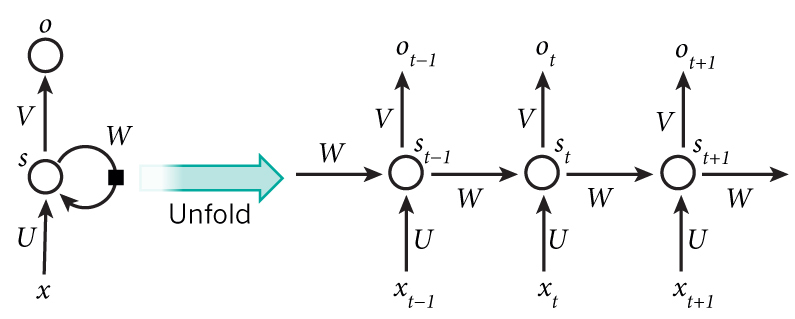
\includegraphics[width=1\linewidth]{images/b3_4.png}
		\label{fig:writing-thesis}
	\end{figure} 

	Mô hình trên mô tả phép triển khai nội dung của một RNN. Triển khai ở đây có thể hiểu đơn giản là ta vẽ ra một mạng nơ-ron chuỗi tuần tự. Ví dụ ta có một câu gồm 5 chữ “Đẹp trai lắm gái theo”, thì mạng nơ-ron được triển khai sẽ gồm 5 tầng nơ-ron tương ứng với mỗi chữ một tầng. 
	
	Đưa vào một chuỗi các tín hiệu âm thanh, ta có thể dự đoán được chuỗi các đoạn ký tự đi kèm với xác xuất của chúng. Ví dụ Hello ~ Helllooooo.
	
	\begin{figure}[H]
		\centering
		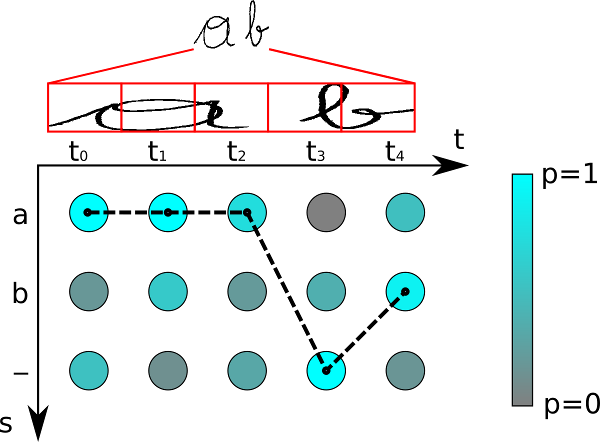
\includegraphics[width=1\linewidth]{images/b3_5.png}
		\label{fig:writing-thesis}
	\end{figure} 
		
	Tư tưởng chủ đạo của phương pháp này chính là tạo ra một mô hình được huấn luyện (CTC : RNN) với đầu vào là dữ liệu giọng nói thô và đầu ra là một bảng ký tự( có thể là ký tự tiếng anh, tiếng la tinh, còn nếu tiếng việt thì cần phải xác định thêm xác suất xuất hiện của dấu câu) kèm theo xác suất xuất hiện của nó theo thời gian. 
	
	Quá trình giải mã sau khi xử lý: Xác định những ký tự có khả năng xuất hiện cao nhất mỗi bước thời gian (có thể là 1s hoặc 2s), Xóa các ký tự bị trùng lặp đồng thời xóa những khoảng trống lặp lại. Phần văn bản còn lại đại diện cho đầu ra.
	
	\begin{figure}[H]
		\centering
		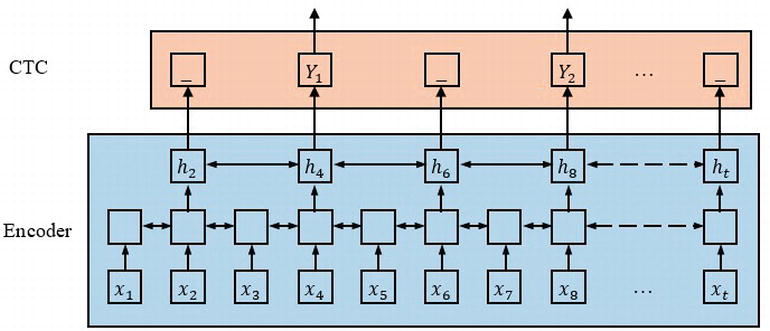
\includegraphics[width=1\linewidth]{images/b3_6.png}
		\label{fig:writing-thesis}
	\end{figure} 


	\begin{figure}[H]
		\centering
		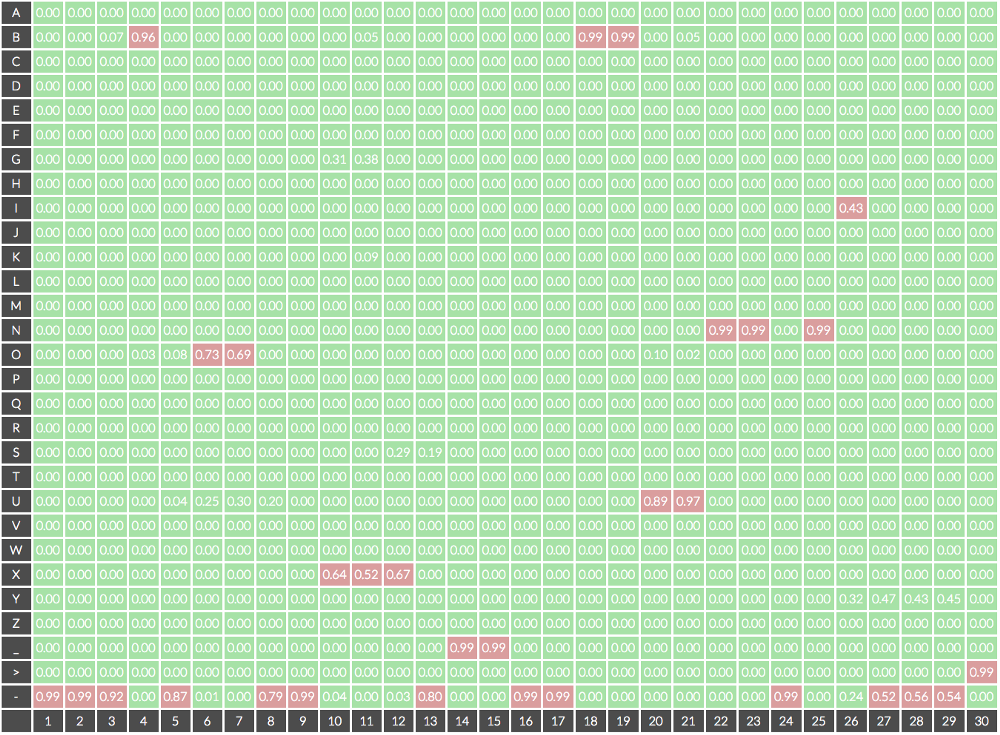
\includegraphics[width=1\linewidth]{images/b3_7.png}
		\label{fig:writing-thesis}
	\end{figure} 

	Quá trình huấn luyện mô hình này có thể được thực hiện theo các bước sau : tính toán xác suất của các alignments bằng cách connect các xác suất của output của các thời điểm lại với nhau và chọn alignment phù hợp nhất, tính sai số của nó và cho network học lại. Vì mô hình này có thể tính toán được hàm loss nên có thể huấn luyện dựa vào gradient descent.
	
	Mô hình RNN được sử dụng cho phương pháp này là vì mô hình này cho đầu ra theo thời gian và mô hình chính trong phương pháp này là mô hình phân loại nào đó mang tính thời gian.
		
	\textbf{Đánh giá mô hình}: Độ phức tạp đơn giản hơn nên thời gian thực hiện mô hình này ngắn hơn so với mô hình CNN ở trên nhưng đưa ra kết quả chưa được tốt. Ưu điểm hơn mô hình này chính là kết quả bám sát theo thời gian nói.
	
	\section{C. Nội dung phân công}
	\begin{center}
		\begin{tabular}{| l | l | l | p{5.5cm} | p{3cm} |}
			\hline
			STT & MSSV & Họ tên & Nội dung công việc & Hoàn thiện (\%)\T\B\\ \hline
			1 & 18120018 & Nguyễn Hoàng Đức & A.5 Kiến thức về mạng nơron sâu (DNN), B-3. Trình bày bài toán thị giác máy tính sử dụng CNNs và RNN & 100\%\T\B \\ \hline
			2 & 18120061 & Lê Nhựt Nam & A-1. Kiến thức về Local Binary Patterns (LBP); A-2. Kiến thức về Principal Component Analysis (PCA) và Linear Discriminant Analysis (LDA); A-4. Kiến thức về mạng nơrồn cơ bản (ANN); B-1. Trình bày  kỹ thuật nhận dạng & 100\%\T\B \\ \hline
			3 & 18120167 & Nguyễn Viết Dũng &  A-3. Kiến thức về Support Vector Machines (SVM); B-2. Trình bày giải pháp nhận dạng trong khoảng thời gian gần đây & 100\%\T\B \\ \hline
		\end{tabular}
	\end{center}
	
	\nocite{*}
	\bibliography{references}\newpage\cleardoublepage
	\bibliographystyle{plain}
\end{document}